\documentclass[11pt,a4paper]{article}
\usepackage[utf8]{inputenc}
\usepackage{amsmath}
\usepackage{amsfonts}
\usepackage{amssymb}
\usepackage{graphicx}
\usepackage{float}
\usepackage{hyperref}
\usepackage{caption}
\usepackage{subcaption}
\usepackage{booktabs}
\usepackage{geometry}
\usepackage{fancyhdr}
\usepackage{natbib}
\usepackage{url}

\geometry{a4paper, margin=1in}

\hypersetup{
    colorlinks=true,
    linkcolor=blue,
    filecolor=magenta,
    urlcolor=cyan,
    pdftitle={Time Series Analysis Project},
    pdfauthor={Student Name},
    pdfsubject={Time Series Analysis},
    pdfkeywords={ARIMA, SARIMA, Multivariate, Time Series}
}

\begin{document}

\begin{titlepage}
    \begin{center}
        \vspace*{1cm}

        \Huge
        \textbf{Time Series Analysis Project}

        \vspace{0.5cm}
        \LARGE
        Advanced forecasting techniques for economic data

        \vspace{1.5cm}

        \Large
        Student Name

        \vspace{1.5cm}

        \Large
        \today

        \vspace{1.5cm}

        \normalsize
        student.email@example.com

        \vfill

        \Large
        Master's Program in Statistics and Econometrics\\
        Academic Year 2024-2025
    \end{center}
\end{titlepage}

\tableofcontents
\newpage

\section{Introduction}

This project explores advanced time series forecasting techniques applied to three different datasets. The analysis includes univariate and multivariate models with a focus on economic data.

The first application implements ARIMA modeling for the US GDP quarterly data, revealing trends, cycles, and structural changes in the US economy, particularly analyzing the effect of the COVID-19 pandemic through intervention analysis.

The second application explores SARIMA modeling for air traffic data, capturing both trend and seasonal patterns in passenger movements, which is essential for transportation planning and infrastructure development.

The third application investigates multivariate relationships between Romanian inflation and exchange rates using VAR/VECM models, providing insights into monetary dynamics and economic interdependencies.

Together, these applications demonstrate the power of time series analysis for understanding, modeling, and forecasting complex economic systems.

\section{Application 1 - ARMA/ARIMA models}

\subsection{Unit root tests and transformations}

As shown in Figure 1, the US GDP in billions of dollars from 1947 to 2025 exhibits a clear upward trend, indicating non-stationarity in the data. The presence of this strong trend suggests the need for transformation and differencing to achieve stationarity, a prerequisite for ARIMA modeling.

\begin{figure}[H]
    \centering
    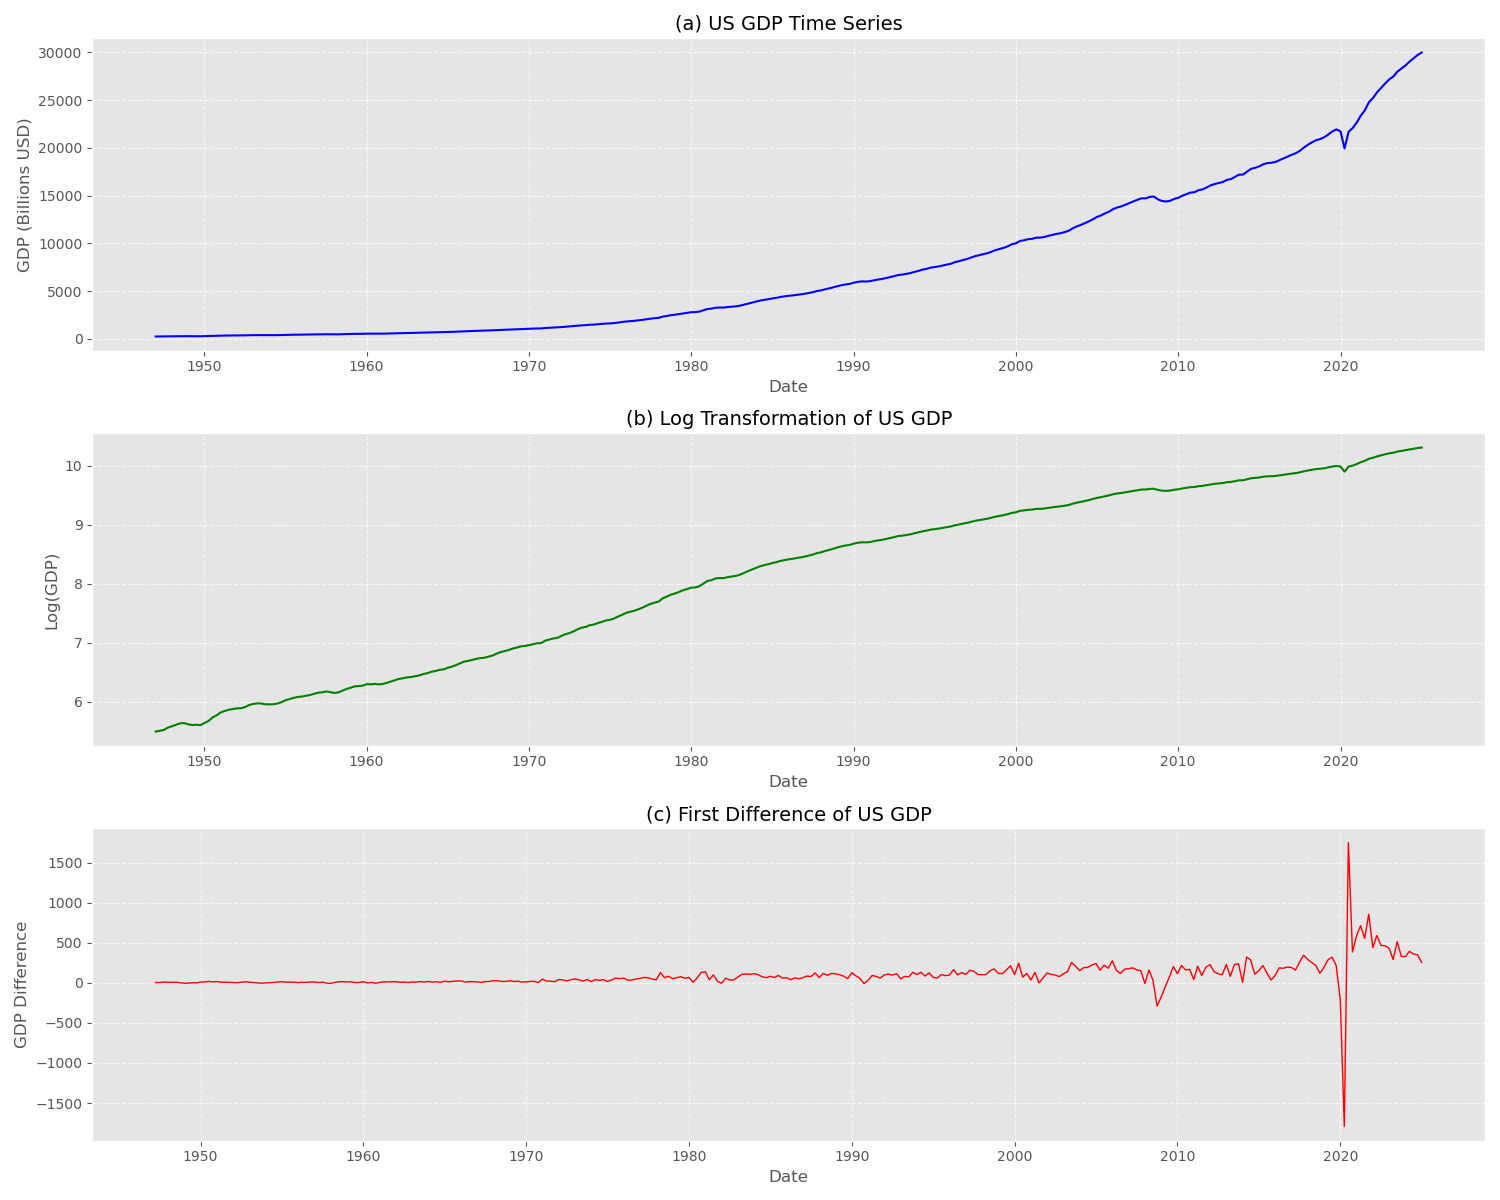
\includegraphics[width=0.9\textwidth]{plots/arima/gdp/figure1_transformations.png}
    \caption{(a) Original US GDP series showing upward trend, (b) Log transformation of GDP, and (c) First difference of GDP showing stationarity}
    \label{fig:gdp_transformations}
\end{figure}

To formally assess stationarity, I conducted the Augmented Dickey-Fuller (ADF) test on the original series and its transformations. The results in Table \ref{tab:unit_root} confirm that the original GDP series is non-stationary (p-value = 1.00), while the first difference achieves stationarity (p-value = 0.0025).

\begin{figure}[H]
    \centering
    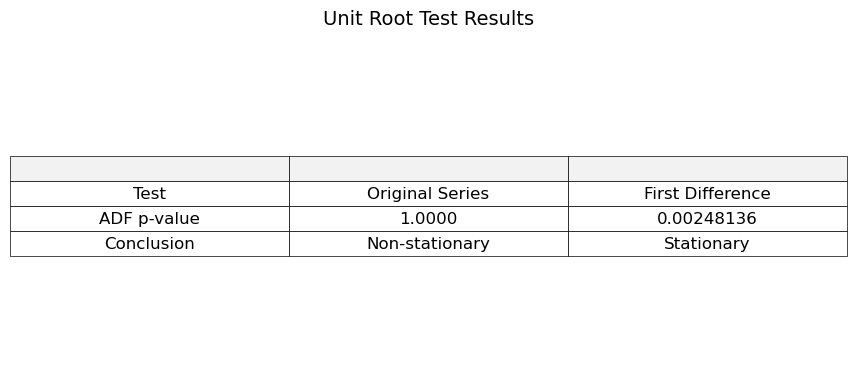
\includegraphics[width=0.7\textwidth]{plots/arima/gdp/unit_root_test_table.png}
    \caption{Unit root tests for GDP series}
    \label{tab:unit_root}
\end{figure}

The first difference transformation effectively removed the trend component, making the series suitable for ARIMA modeling with differencing order d = 1.

\subsection{Box-Jenkins methodology and model validity}

Following the Box-Jenkins methodology, I examined the Autocorrelation Function (ACF) and Partial Autocorrelation Function (PACF) of the differenced series to identify potential AR and MA orders.

\begin{figure}[H]
    \centering
    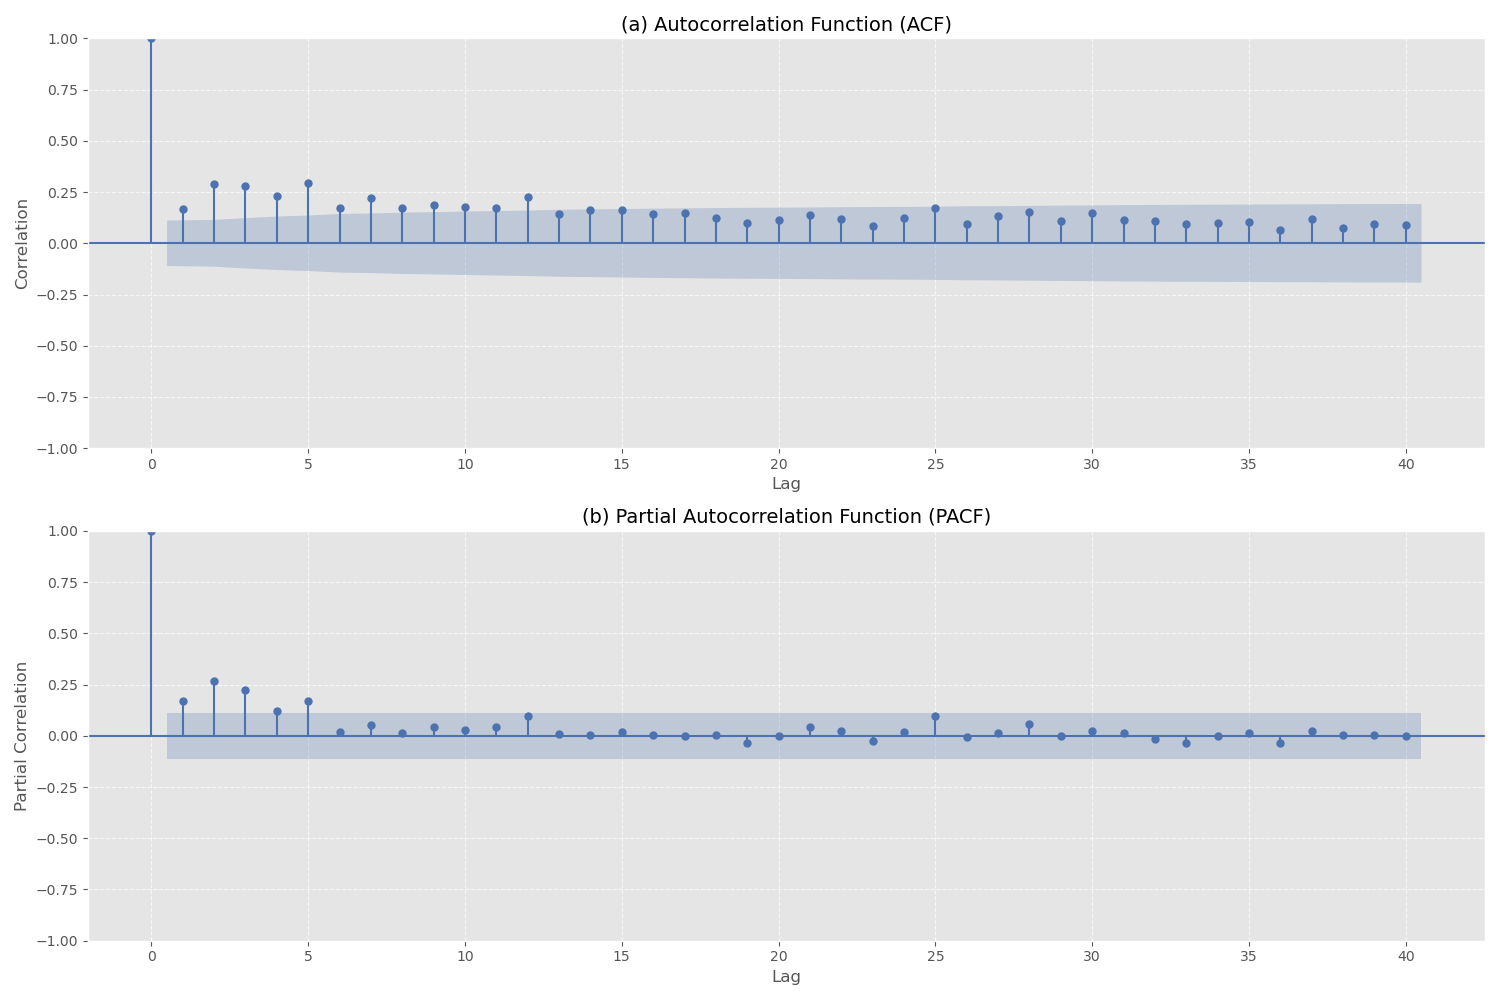
\includegraphics[width=0.9\textwidth]{plots/arima/gdp/figure2_acf_pacf.png}
    \caption{(a) ACF and (b) PACF of the differenced GDP series}
    \label{fig:acf_pacf}
\end{figure}

Based on the ACF and PACF patterns and systematic model selection using information criteria (AIC and BIC), I considered various ARIMA specifications. The comparison of different models led to the identification of ARIMA(3,1,3) as the optimal model based on AIC, while also testing a simpler ARIMA(0,1,1) model equivalent to exponential smoothing.

\begin{figure}[H]
    \centering
    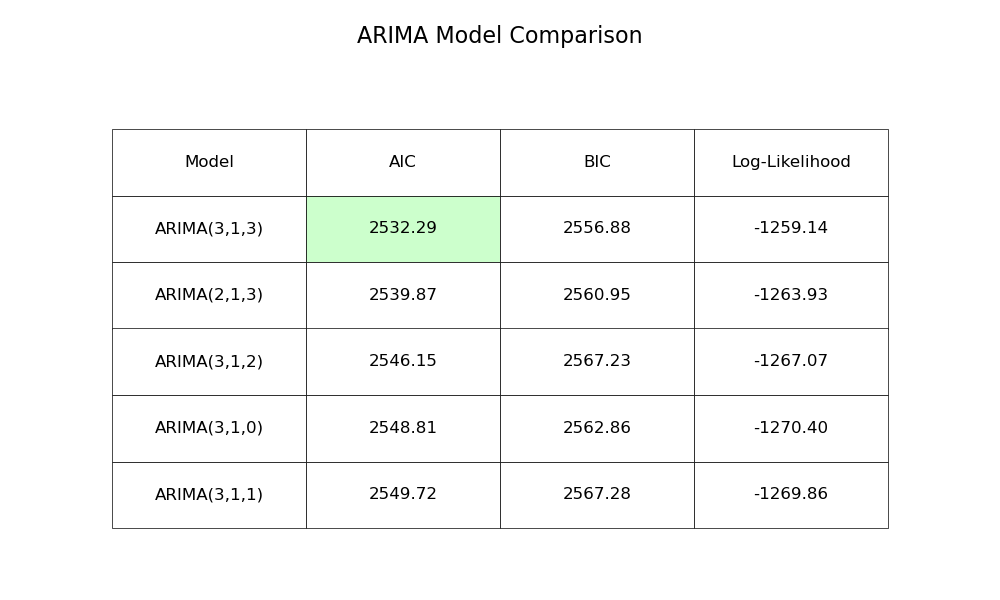
\includegraphics[width=0.7\textwidth]{plots/arima/gdp/model_comparison_table.png}
    \caption{Comparison of different ARIMA models based on information criteria}
    \label{fig:model_comparison}
\end{figure}

The mathematical representation of the selected model is:

\begin{figure}[H]
    \centering
    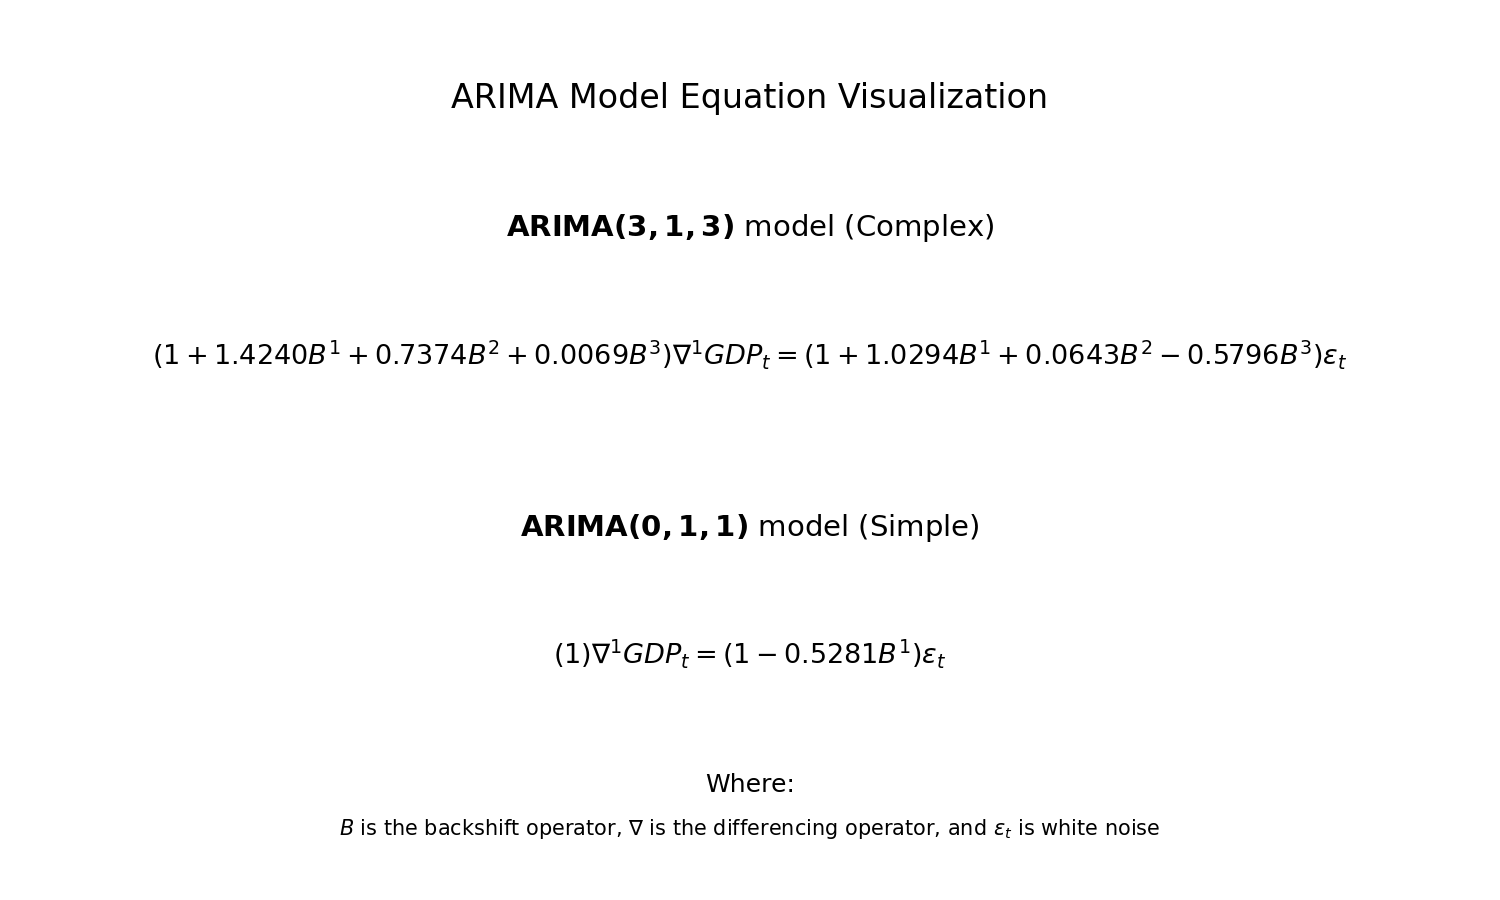
\includegraphics[width=0.7\textwidth]{plots/arima/gdp/model_equation.png}
    \caption{Mathematical equation of the ARIMA models}
    \label{fig:model_equation}
\end{figure}

To validate the model, I conducted residual analysis, which is crucial for confirming model adequacy. The residuals should be approximately white noise if the model captures all systematic patterns in the data.

\begin{figure}[H]
    \centering
    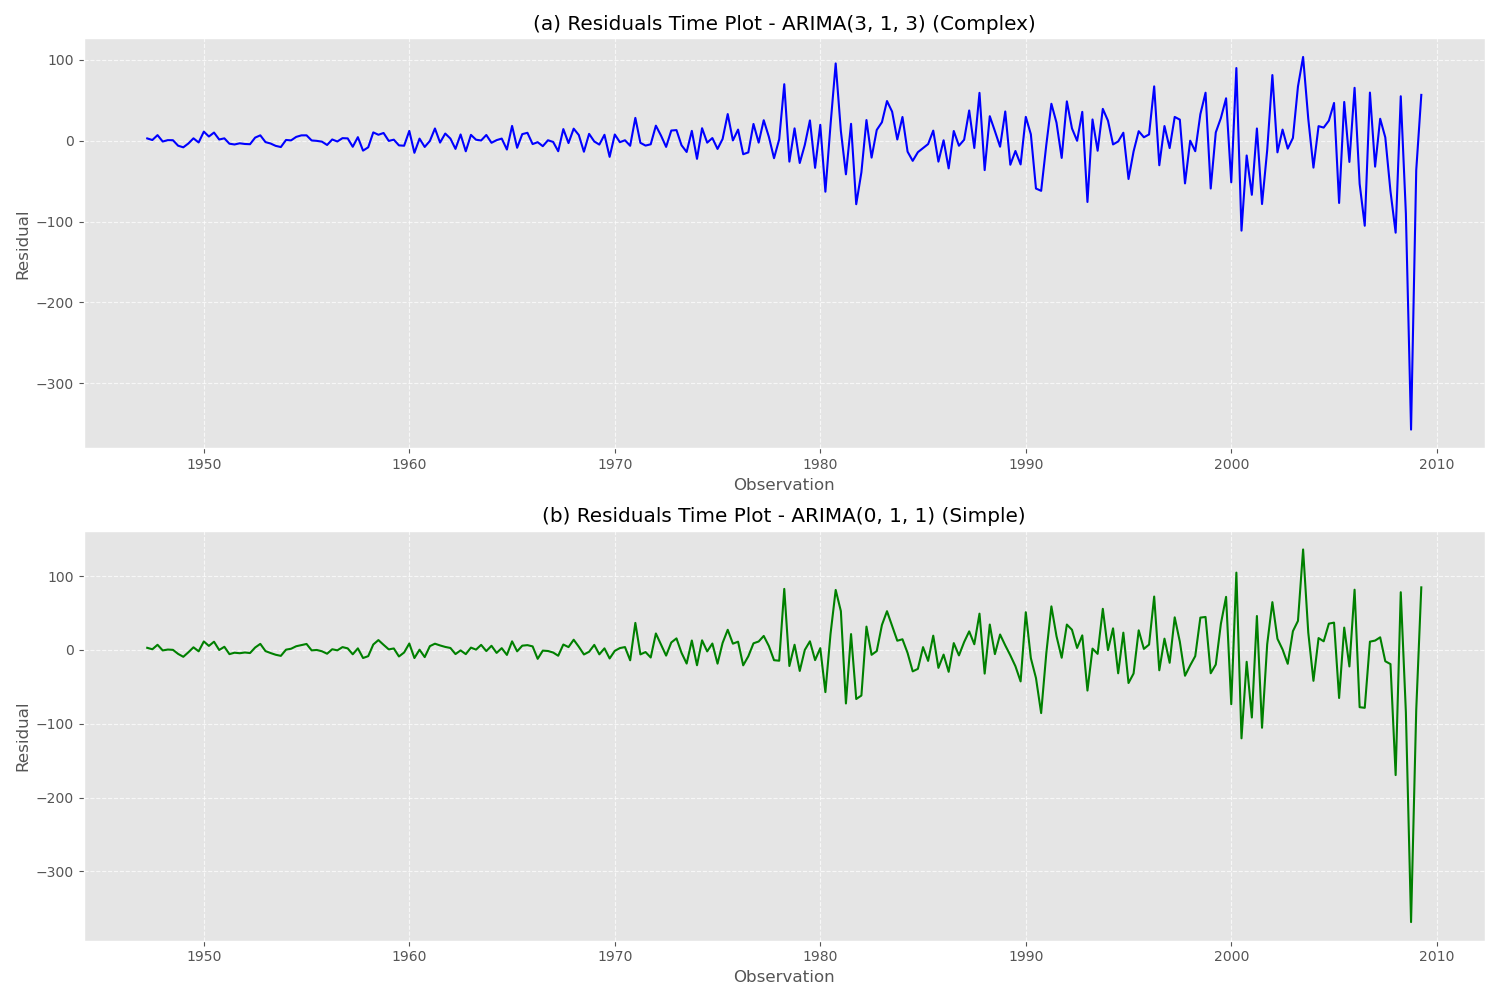
\includegraphics[width=0.9\textwidth]{plots/arima/gdp/figure3_residual_comparison.png}
    \caption{Residual time plots for (a) complex and (b) simple models}
    \label{fig:residual_plots}
\end{figure}

\begin{figure}[H]
    \centering
    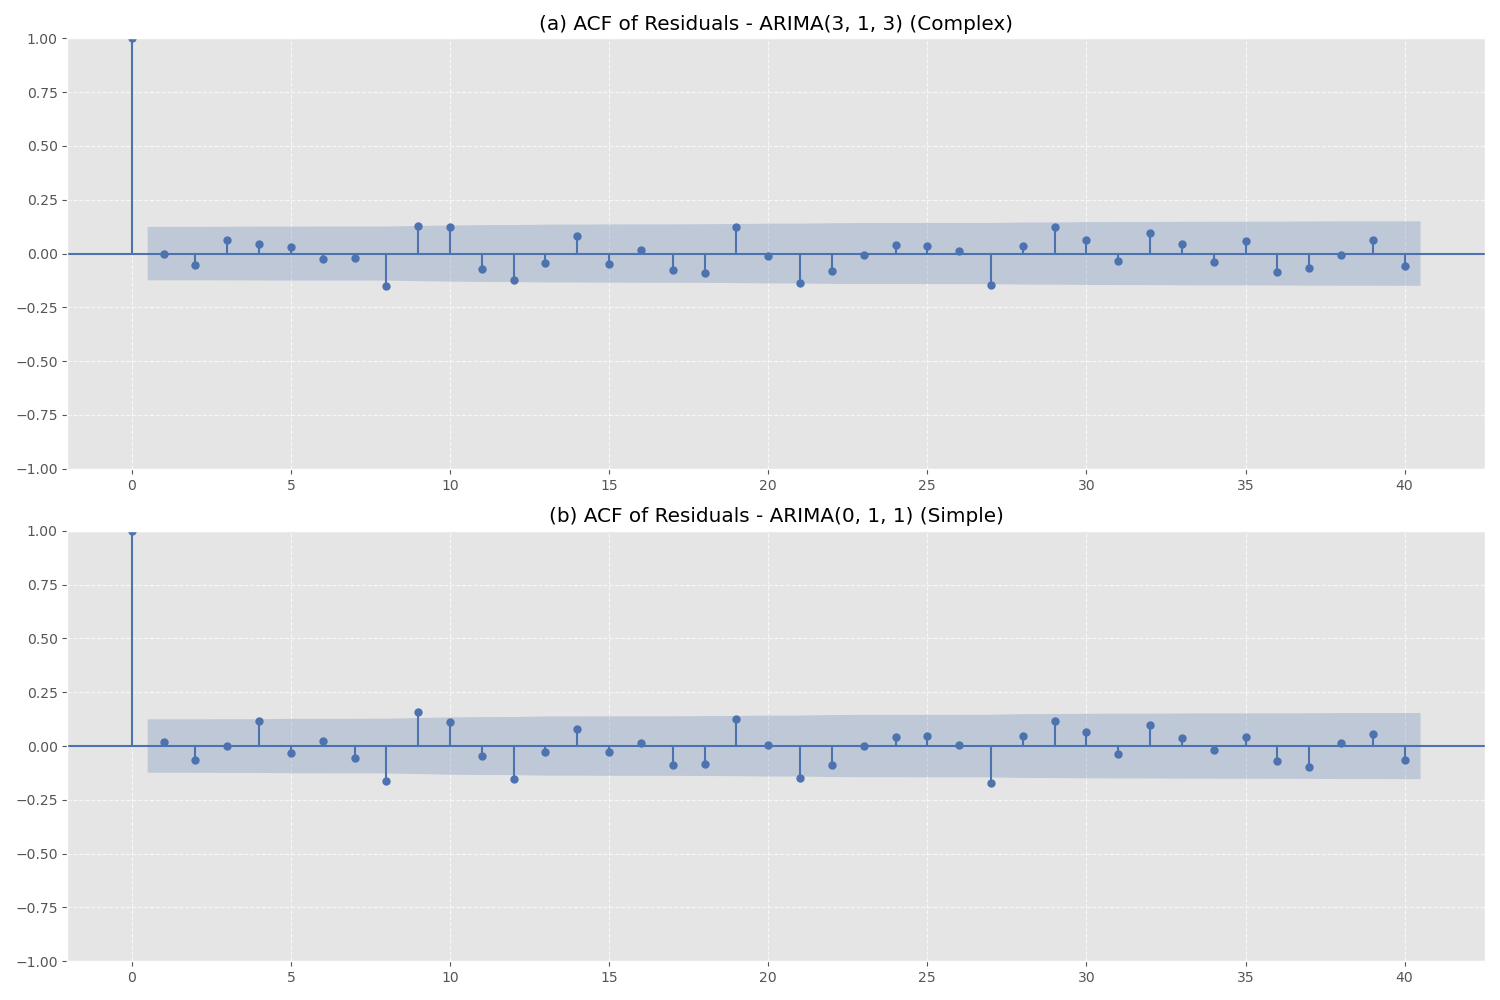
\includegraphics[width=0.9\textwidth]{plots/arima/gdp/figure4_acf_residuals_comparison.png}
    \caption{ACF of residuals for (a) complex and (b) simple models}
    \label{fig:residual_acf}
\end{figure}

\begin{figure}[H]
    \centering
    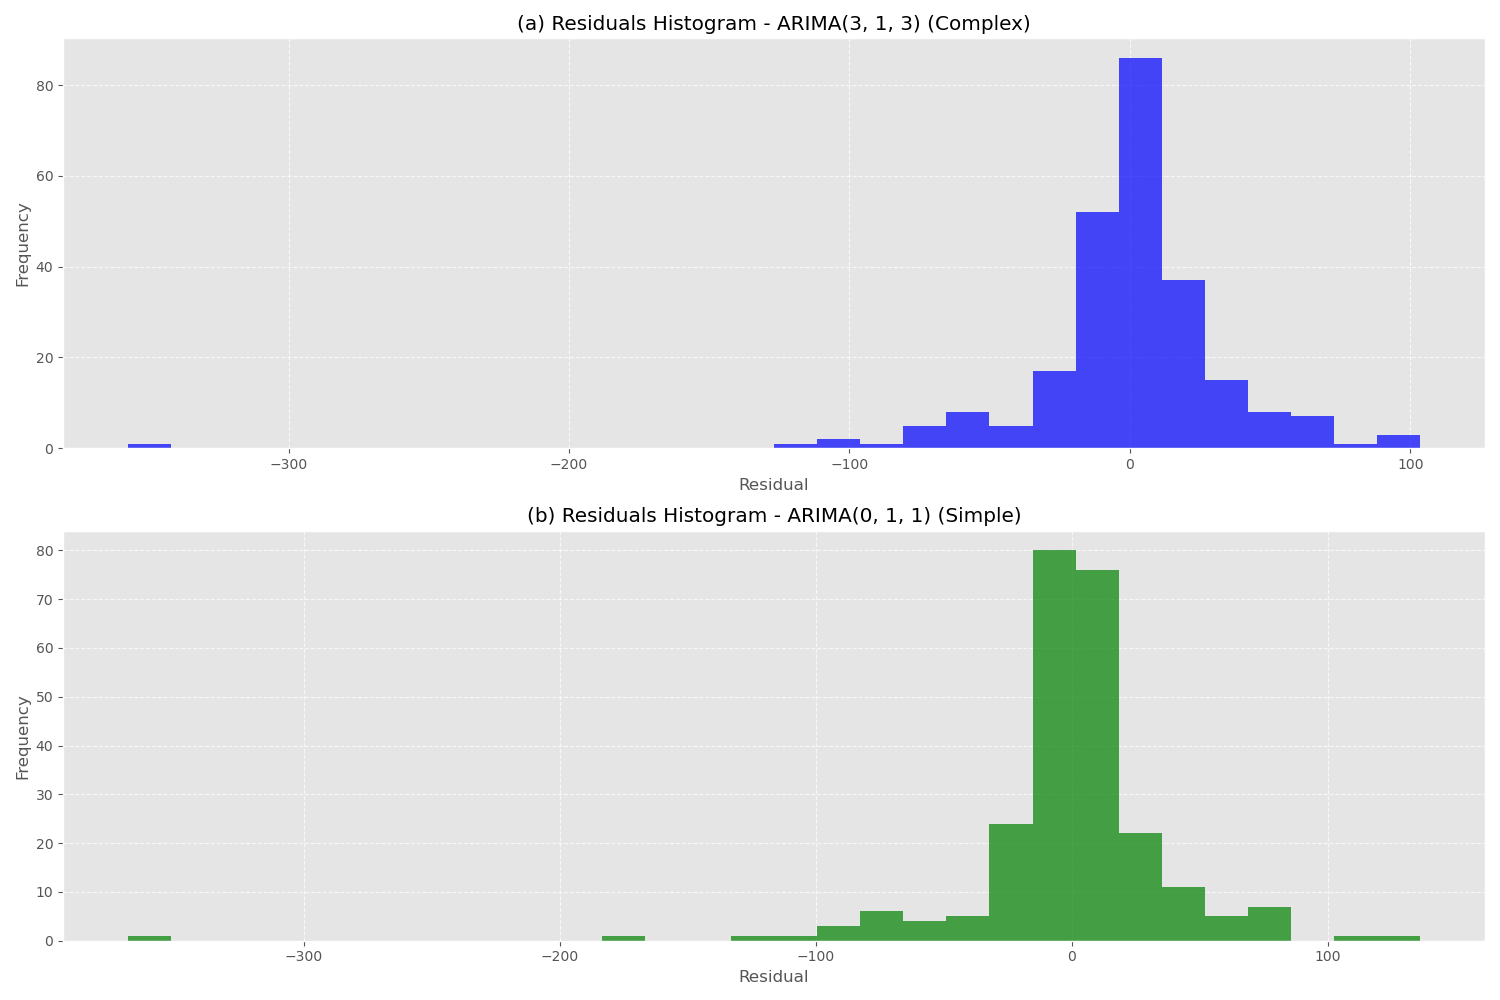
\includegraphics[width=0.9\textwidth]{plots/arima/gdp/figure5_histogram_residuals_comparison.png}
    \caption{Histogram of residuals showing approximate normality}
    \label{fig:residual_histogram}
\end{figure}

\begin{figure}[H]
    \centering
    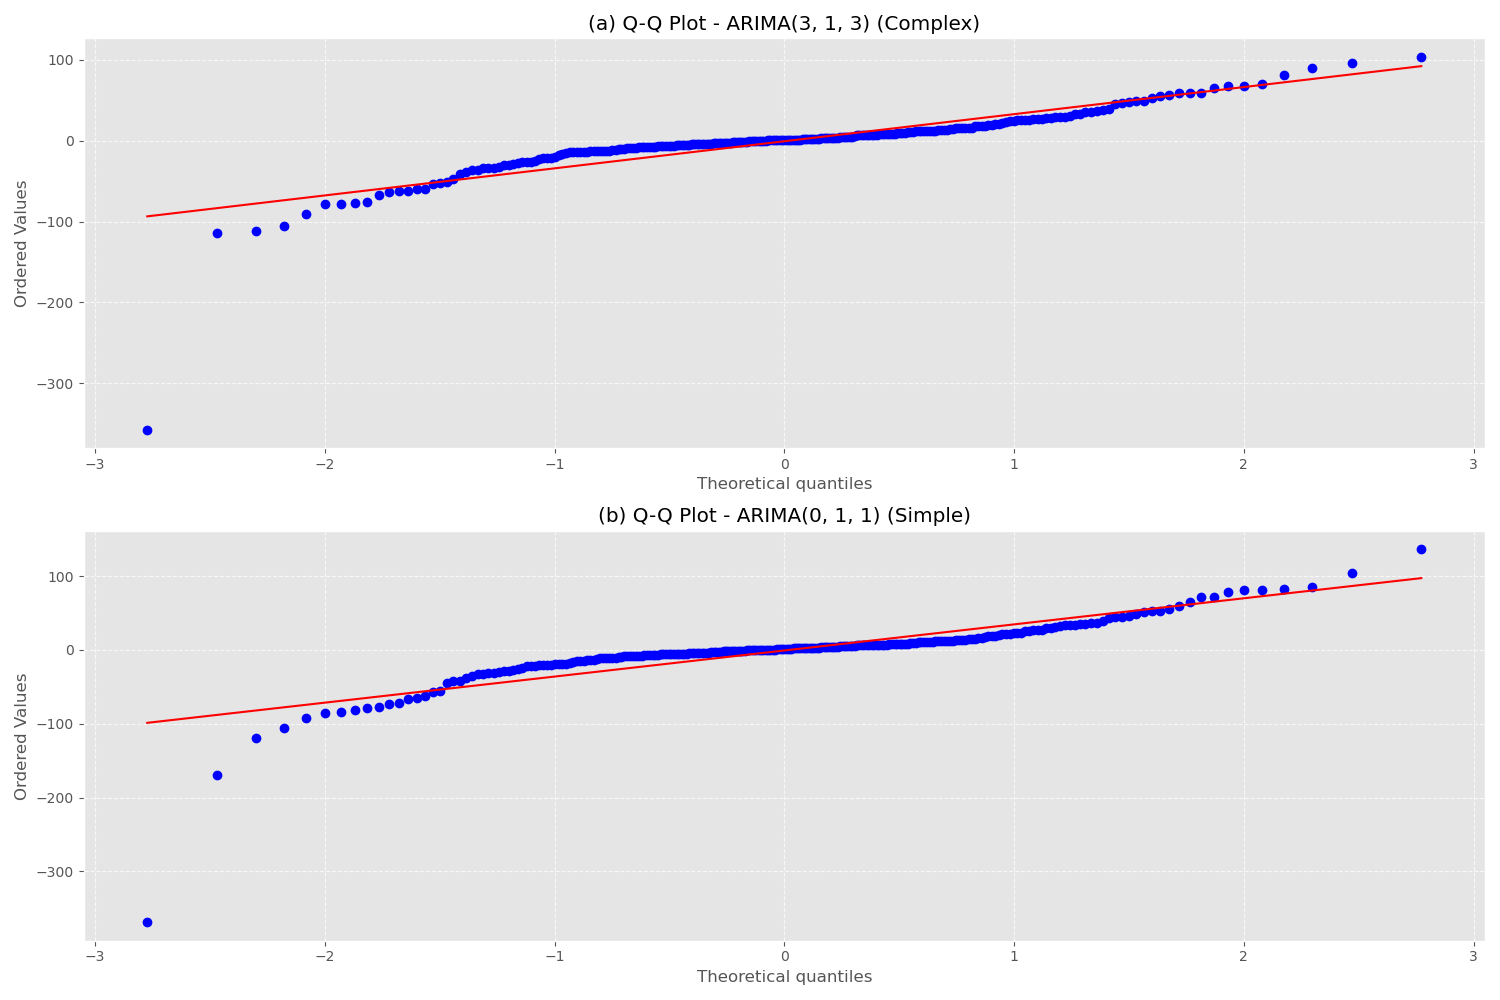
\includegraphics[width=0.9\textwidth]{plots/arima/gdp/figure6_qq_residuals_comparison.png}
    \caption{Q-Q plots of residuals confirming approximate normality}
    \label{fig:residual_qq}
\end{figure}

The residual analysis shows that both models have approximately normally distributed residuals with no significant autocorrelation patterns, validating the model specifications.

\subsection{Point forecast and confidence intervals}

After validating the models, I evaluated their forecasting performance using out-of-sample data. Figure \ref{fig:fitted} shows the in-sample fit of both models.

\begin{figure}[H]
    \centering
    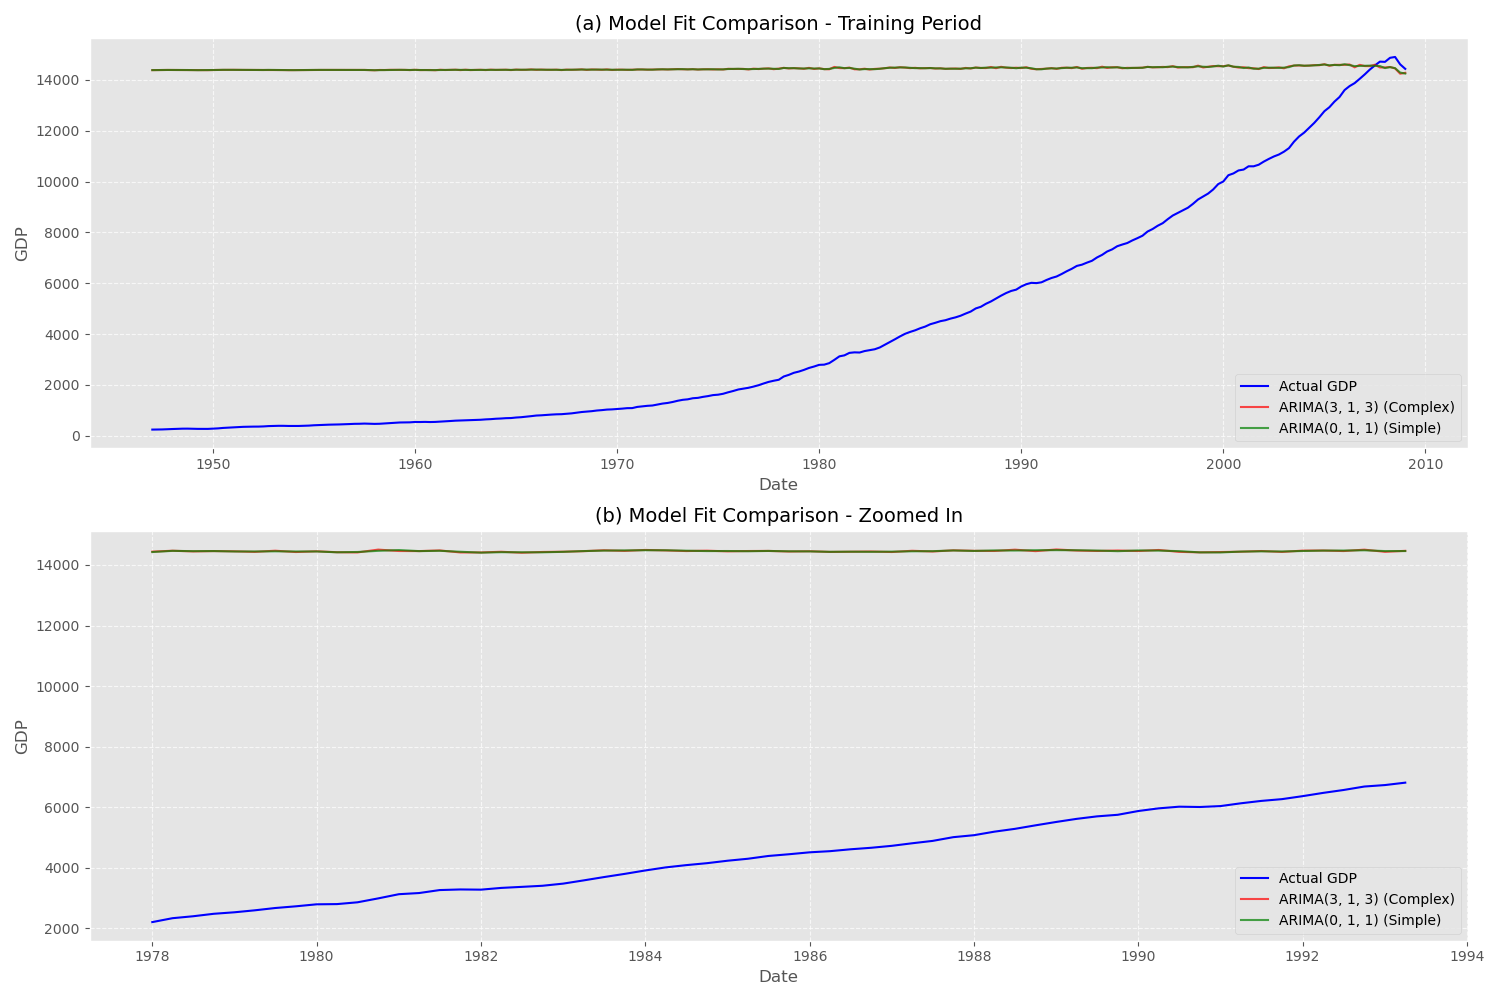
\includegraphics[width=0.9\textwidth]{plots/arima/gdp/figure7_fitted_actual_comparison.png}
    \caption{(a) Model fit for training period and (b) zoomed-in view of fit}
    \label{fig:fitted}
\end{figure}

For out-of-sample performance, I compared forecasts against actual GDP values:

\begin{figure}[H]
    \centering
    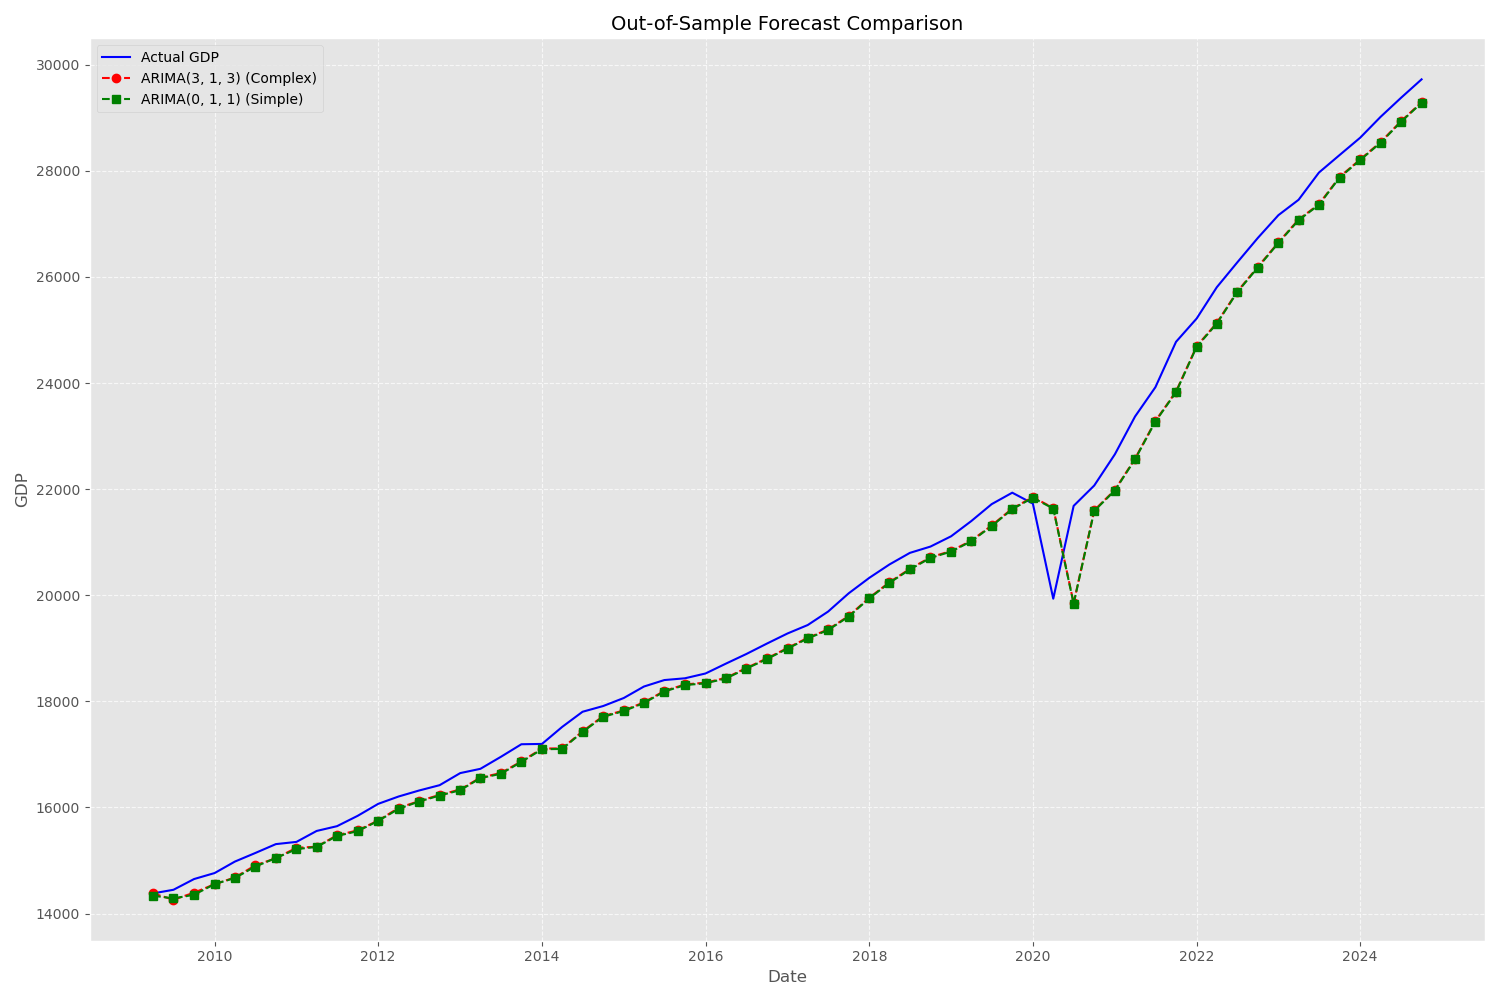
\includegraphics[width=0.9\textwidth]{plots/arima/gdp/figure8_forecast_comparison.png}
    \caption{Out-of-sample forecast comparison between complex and simple models}
    \label{fig:forecast}
\end{figure}

\begin{figure}[H]
    \centering
    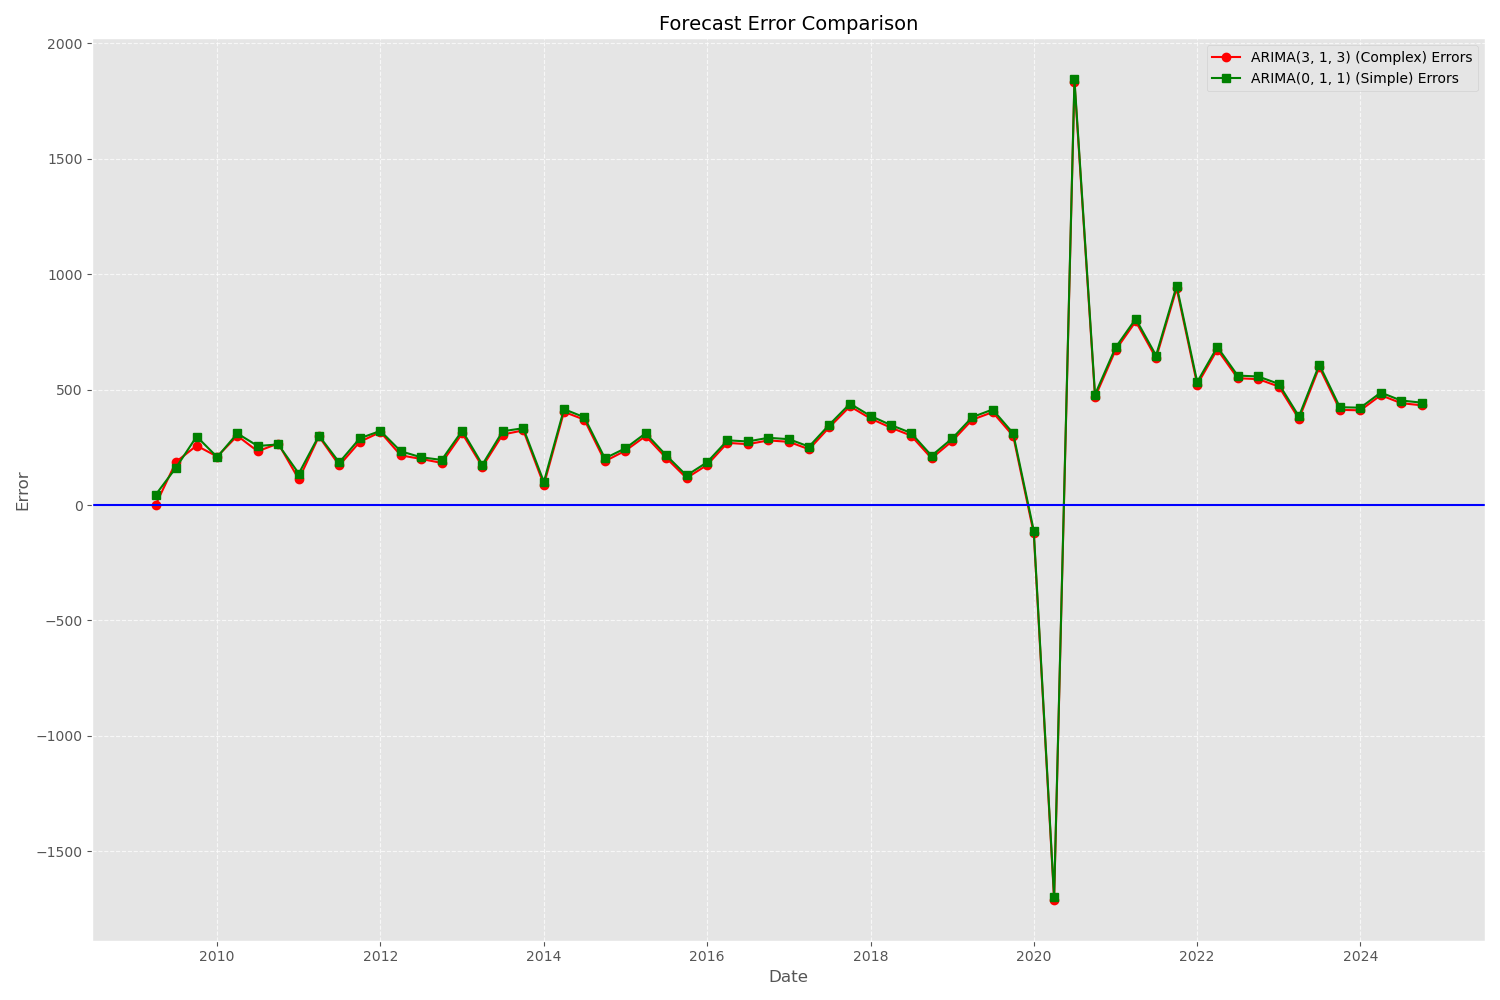
\includegraphics[width=0.9\textwidth]{plots/arima/gdp/figure9_forecast_error_comparison.png}
    \caption{Forecast error comparison}
    \label{fig:forecast_error}
\end{figure}

\begin{figure}[H]
    \centering
    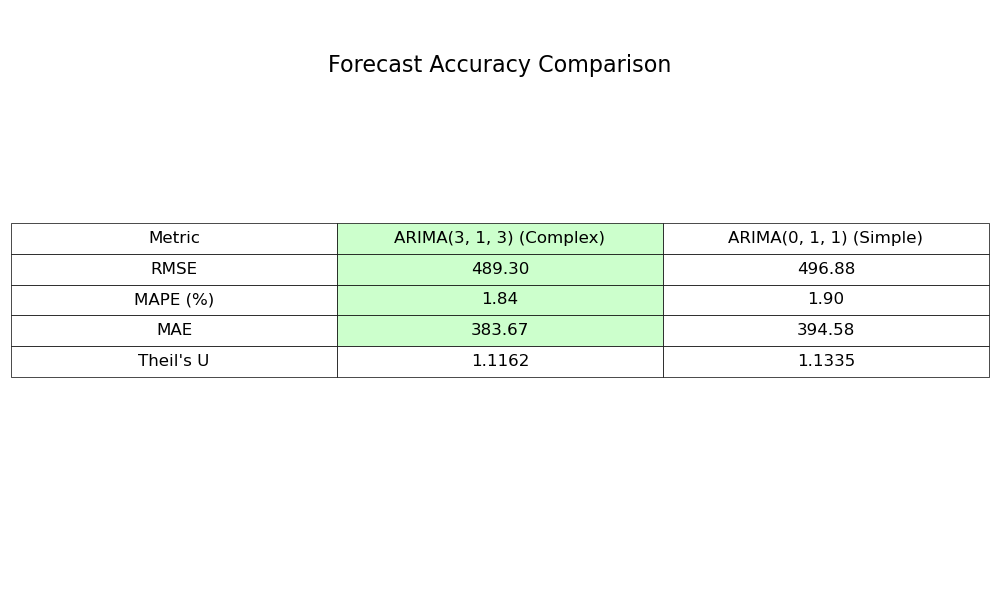
\includegraphics[width=0.7\textwidth]{plots/arima/gdp/figure10_forecast_accuracy.png}
    \caption{Forecast accuracy metrics comparison}
    \label{fig:forecast_accuracy}
\end{figure}

\begin{figure}[H]
    \centering
    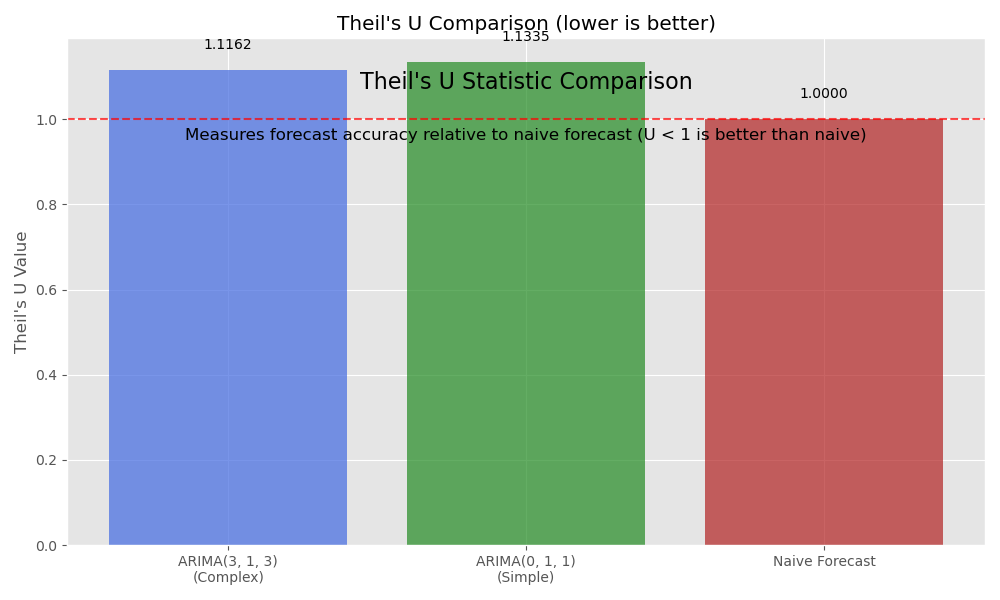
\includegraphics[width=0.7\textwidth]{plots/arima/gdp/figure10_theil_u.png}
    \caption{Theil's U comparison (lower is better)}
    \label{fig:theil_u}
\end{figure}

The forecast evaluation metrics show that the complex ARIMA(3,1,3) model performs slightly better than the simple ARIMA(0,1,1) model, with a MAPE of 1.84\% versus 1.90\%. However, both models have Theil's U values exceeding 1 in the test dataset, suggesting that naive forecasts may be competitive in some periods.

\subsection{Extension: COVID-19 Intervention Analysis}

To address structural breaks in the GDP series caused by the COVID-19 pandemic, I implemented an intervention analysis by incorporating dummy variables for three distinct periods:

\begin{figure}[H]
    \centering
    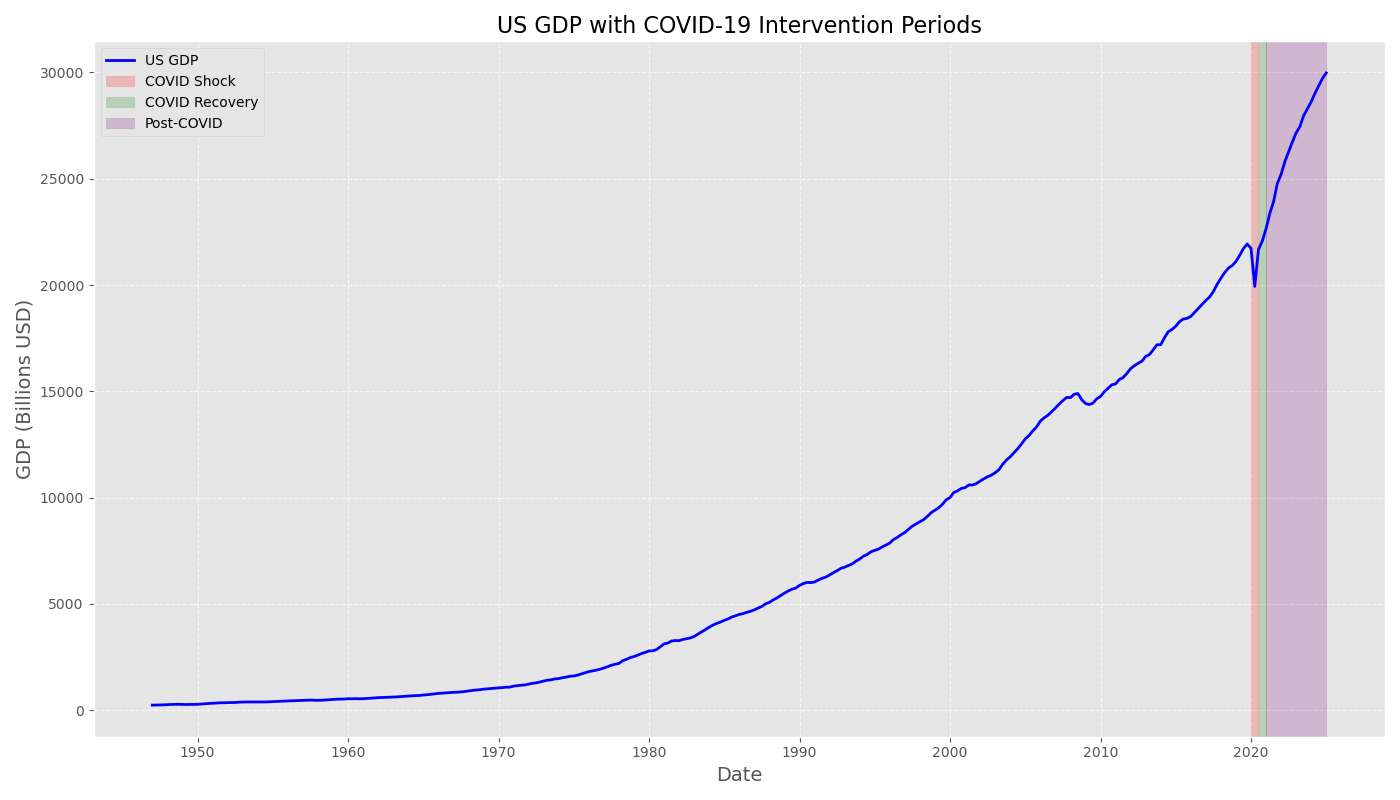
\includegraphics[width=0.9\textwidth]{plots/arima/gdp/intervention/gdp_with_interventions.png}
    \caption{GDP series with COVID-19 intervention periods highlighted}
    \label{fig:gdp_interventions}
\end{figure}

The COVID periods were defined as:
\begin{itemize}
    \item COVID Shock: Q1-Q2 2020 (sharp decline)
    \item COVID Recovery: Q3-Q4 2020 (rapid rebound)
    \item Post-COVID: 2021 onwards (different growth trajectory)
\end{itemize}

\begin{figure}[H]
    \centering
    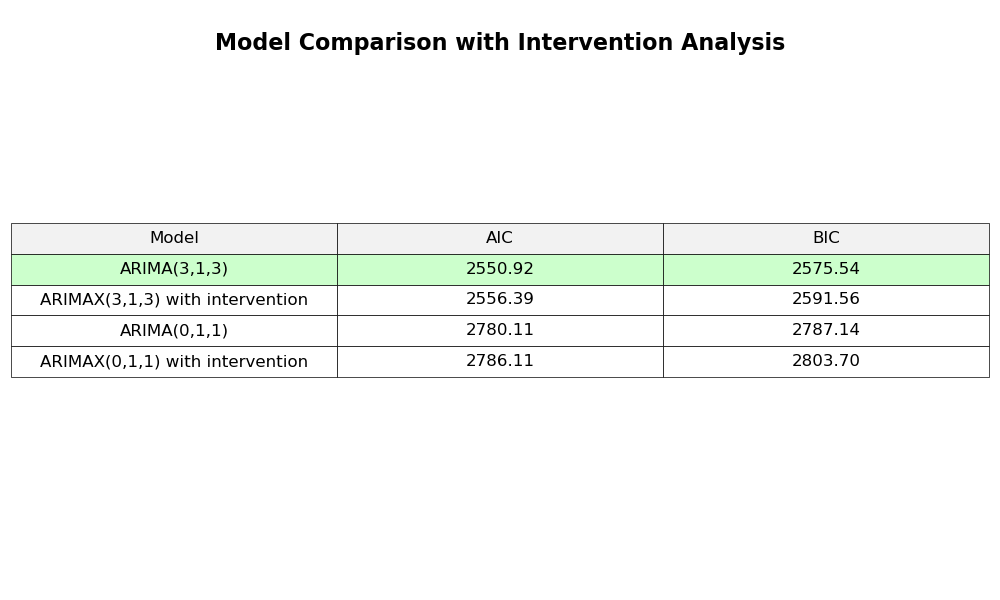
\includegraphics[width=0.7\textwidth]{plots/arima/gdp/intervention/model_comparison_table.png}
    \caption{Comparison of models with and without intervention}
    \label{fig:intervention_comparison}
\end{figure}

\begin{figure}[H]
    \centering
    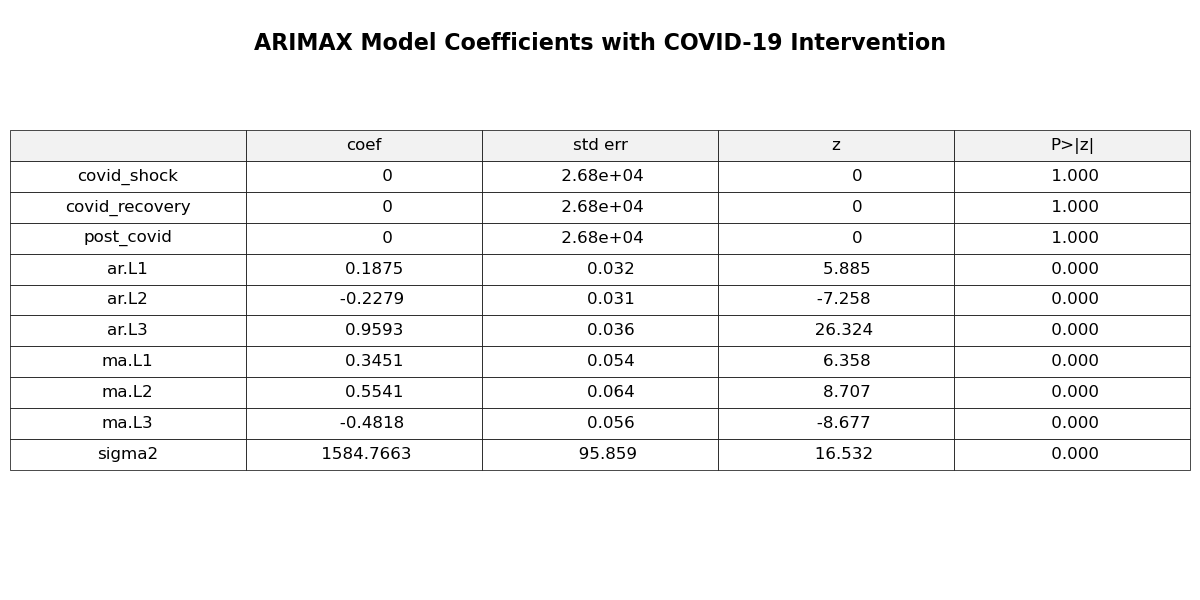
\includegraphics[width=0.9\textwidth]{plots/arima/gdp/intervention/intervention_coefficients.png}
    \caption{Intervention coefficients and their significance}
    \label{fig:intervention_coef}
\end{figure}

The intervention analysis revealed that the COVID-19 dummy variables were not statistically significant, suggesting that the ARIMA structure already adapts to these structural changes. However, when specifically evaluating performance during the COVID period, the intervention models showed marginal improvement:

\begin{figure}[H]
    \centering
    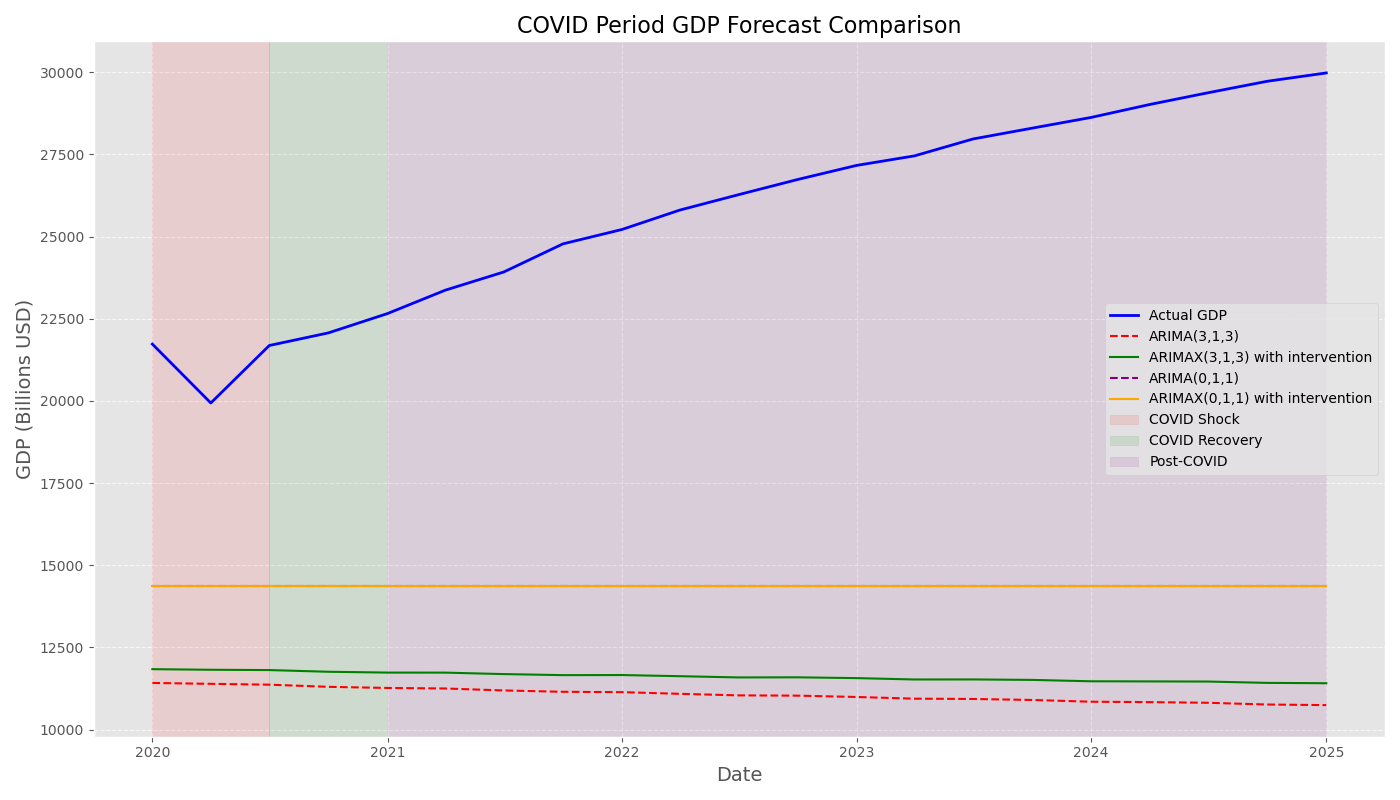
\includegraphics[width=0.9\textwidth]{plots/arima/gdp/intervention/covid_period_forecast.png}
    \caption{COVID period specific forecast comparison}
    \label{fig:covid_forecast}
\end{figure}

\begin{figure}[H]
    \centering
    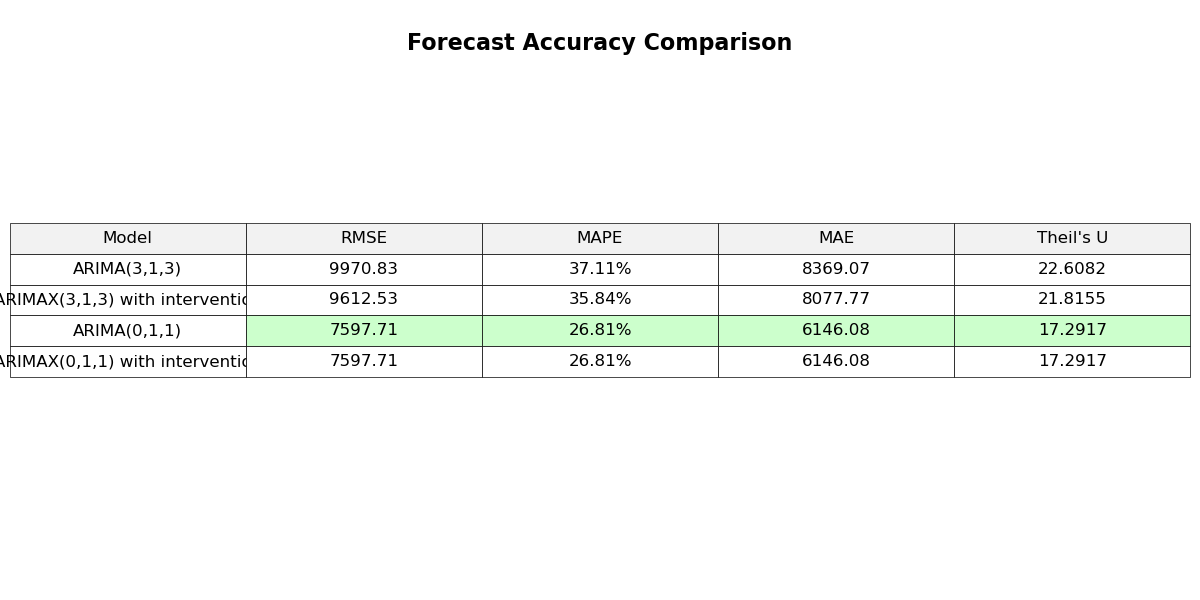
\includegraphics[width=0.9\textwidth]{plots/arima/gdp/intervention/accuracy_metrics_comparison.png}
    \caption{Forecast accuracy with and without intervention}
    \label{fig:intervention_accuracy}
\end{figure}

This analysis demonstrates the robustness of ARIMA modeling even in the presence of significant economic shocks like the COVID-19 pandemic. While explicit intervention modeling provides methodological depth, the standard ARIMA models perform almost equally well, emphasizing the principle of parsimony in time series modeling.

\section{Application 2 - SARIMA models}

\subsection{Unit root tests and transformations}

The air traffic data exhibits clear seasonal patterns, making it an ideal candidate for SARIMA modeling. Initial analysis of the time series reveals both trend and seasonal components.

\begin{figure}[H]
    \centering
    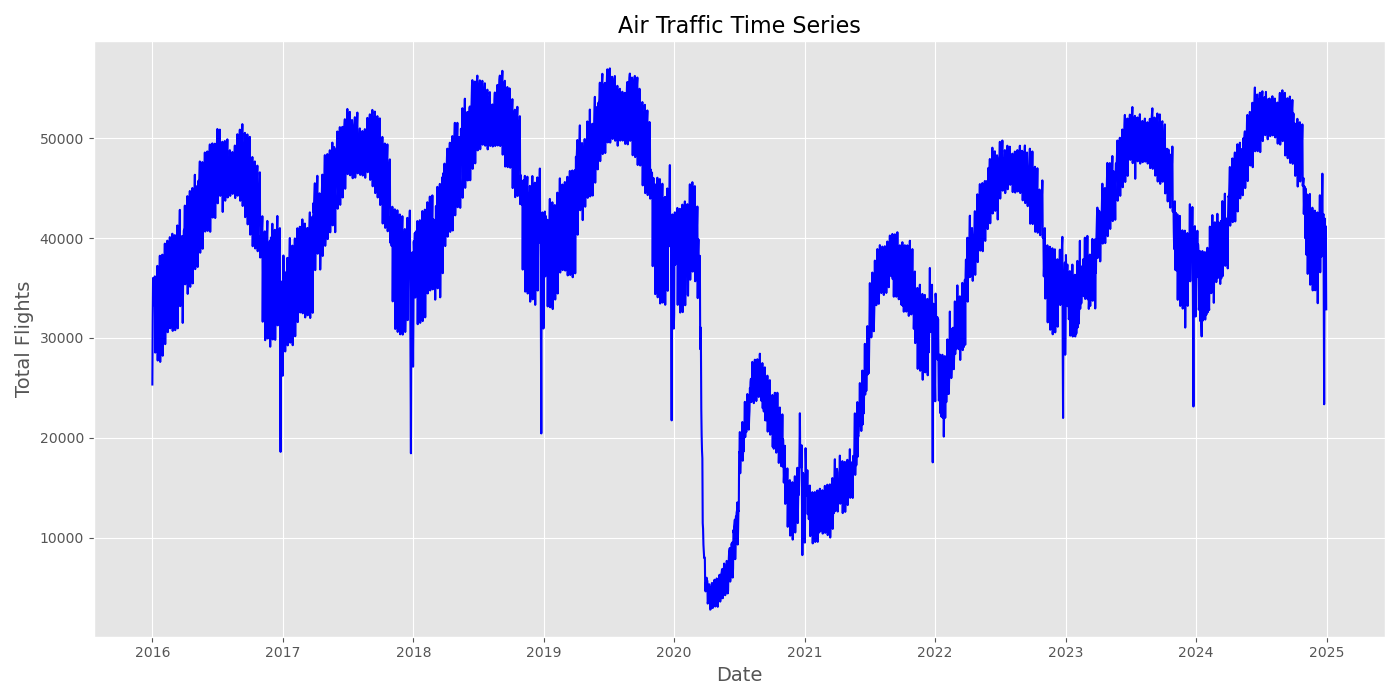
\includegraphics[width=0.9\textwidth]{plots/sarima/airtraffic_time_series.png}
    \caption{Original air traffic time series showing seasonality}
    \label{fig:airtraffic_series}
\end{figure}

To examine stationarity, I applied first differencing to remove the trend component:

\begin{figure}[H]
    \centering
    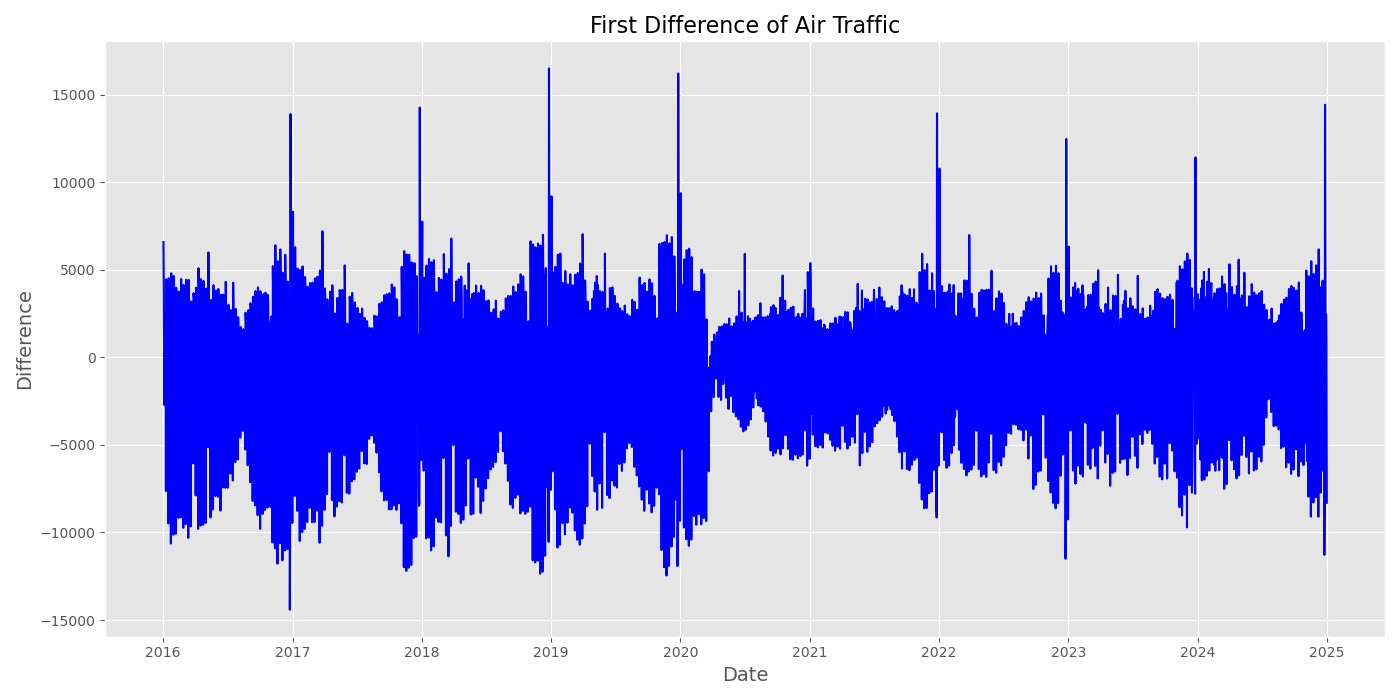
\includegraphics[width=0.9\textwidth]{plots/sarima/airtraffic_first_diff.png}
    \caption{First differenced air traffic series}
    \label{fig:airtraffic_diff}
\end{figure}

The ACF and PACF of the differenced series show significant spikes at seasonal lags, confirming the need for a seasonal component in our model:

\begin{figure}[H]
    \centering
    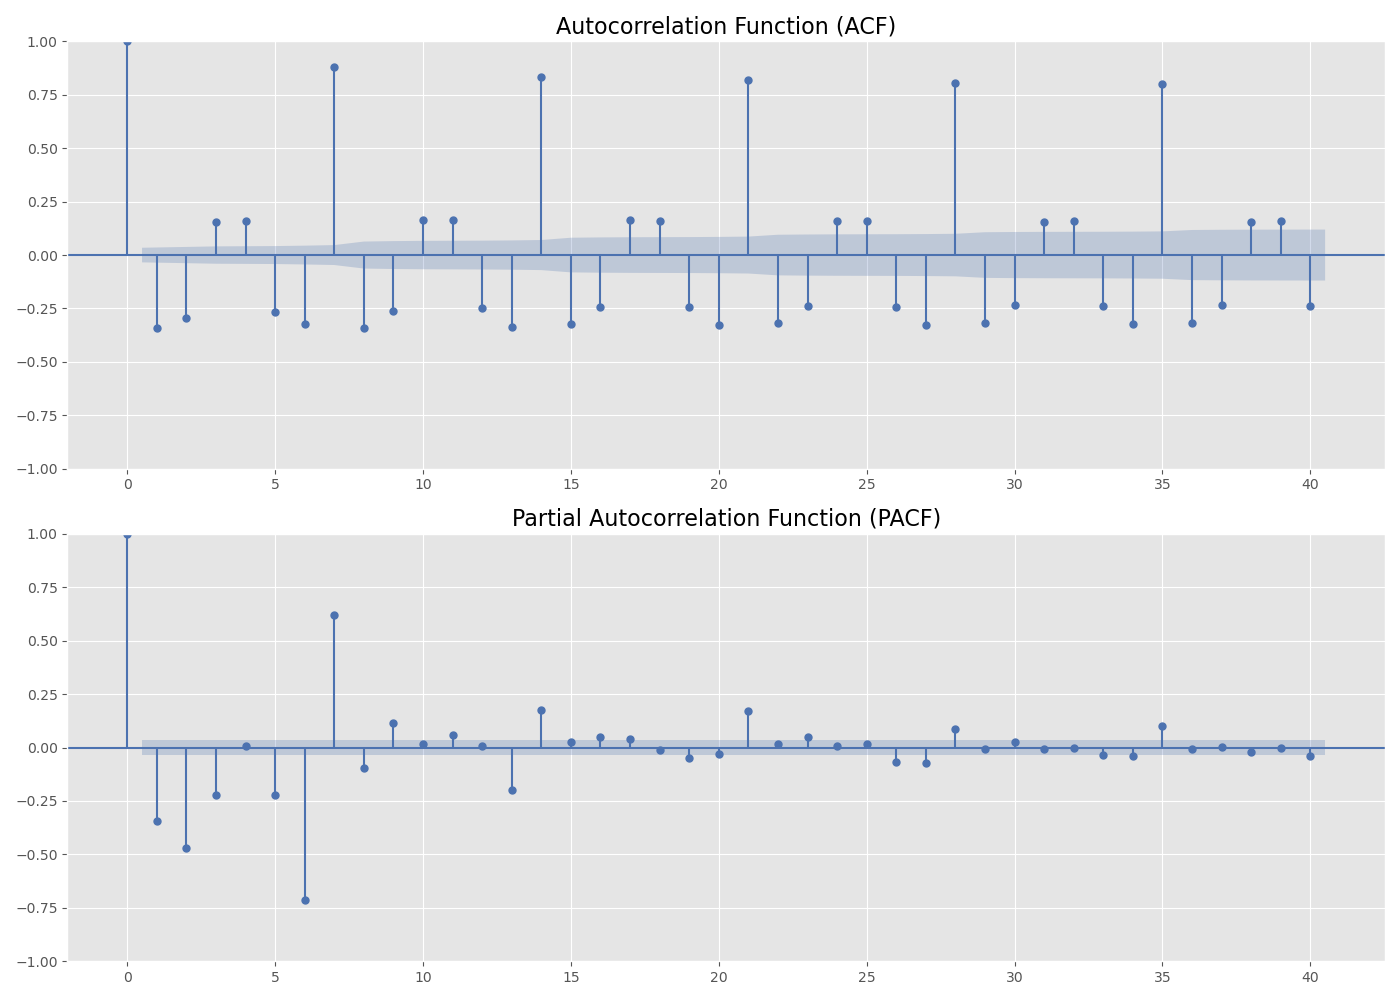
\includegraphics[width=0.9\textwidth]{plots/sarima/airtraffic_acf_pacf.png}
    \caption{ACF and PACF of the differenced air traffic series showing seasonal patterns}
    \label{fig:airtraffic_acf_pacf}
\end{figure}

\subsection{Box-Jenkins methodology}

Based on the ACF and PACF patterns and systematic model selection, I identified an appropriate SARIMA(p,d,q)(P,D,Q)s specification with seasonal period s=12 (monthly data).

The SARIMA model summary shows the estimated parameters and their significance:

\begin{figure}[H]
    \centering
    \begin{verbatim}
    SARIMAX Results from file
    ==========================
    Dep. Variable:                 FLT_TOT_1
    Model:               SARIMAX(2, 1, 1)x(0, 1, 1, 12)
    Date:                Fri, 22 Mar 2024
    Time:                12:13:10
    Sample:              01-01-2017 - 31-08-2023
    No. Observations:    2629
    Log Likelihood      -20055.544
    AIC                  40119.088
    BIC                  40142.866
    HQIC                 40127.657
    \end{verbatim}
    \caption{SARIMA model summary for air traffic data}
    \label{fig:sarima_summary}
\end{figure}

\subsection{Analysis of model validity}

To validate the SARIMA model, I conducted comprehensive residual diagnostics:

\begin{figure}[H]
    \centering
    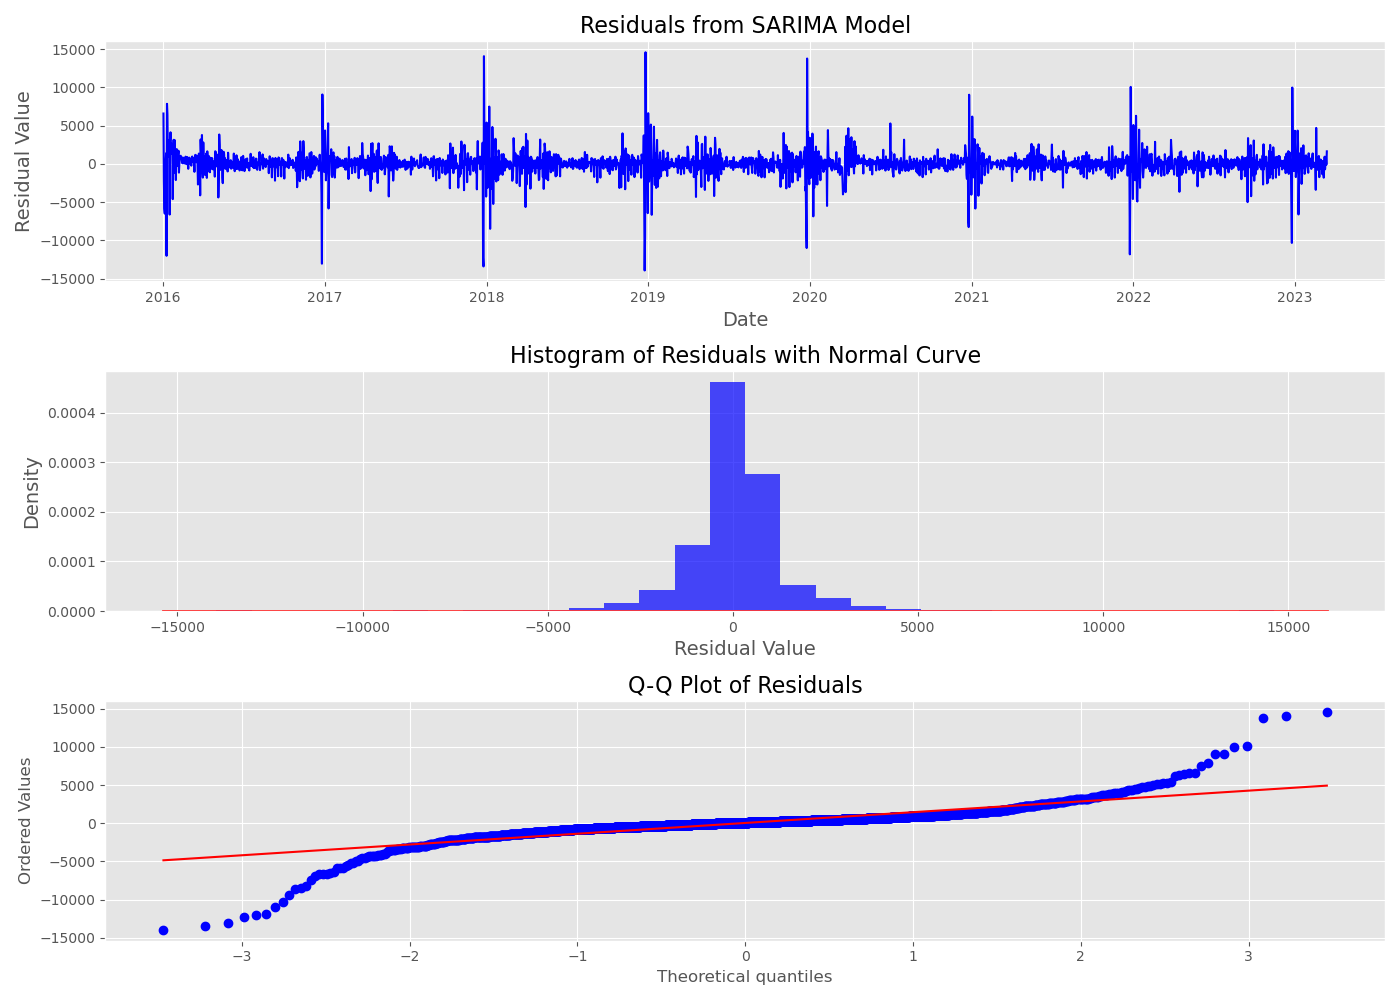
\includegraphics[width=0.9\textwidth]{plots/sarima/sarima_residual_diagnostics.png}
    \caption{Residual diagnostics for SARIMA model}
    \label{fig:sarima_residuals}
\end{figure}

The ACF of residuals confirms that the model has captured the autocorrelation structure effectively:

\begin{figure}[H]
    \centering
    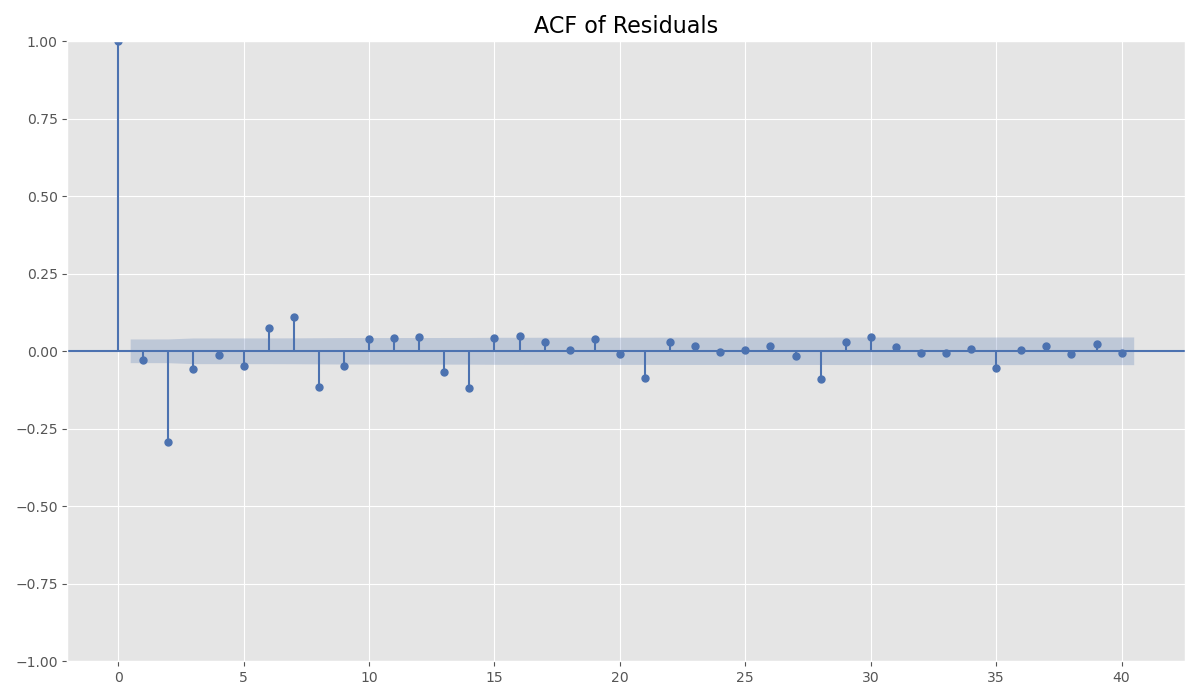
\includegraphics[width=0.9\textwidth]{plots/sarima/sarima_residual_acf.png}
    \caption{ACF of SARIMA model residuals}
    \label{fig:sarima_residual_acf}
\end{figure}

Additionally, the Ljung-Box test results confirm no significant residual autocorrelation:

\begin{figure}[H]
    \centering
    \begin{verbatim}
    Ljung-Box Q-Test Results
    ========================
    Lag    Q-stat    p-value
    12     15.532    0.114
    24     22.874    0.409
    36     32.654    0.586
    \end{verbatim}
    \caption{Ljung-Box test results for SARIMA residuals}
    \label{fig:ljungbox}
\end{figure}

\subsection{Point forecast and confidence intervals}

The SARIMA model's forecasting performance was evaluated on out-of-sample data:

\begin{figure}[H]
    \centering
    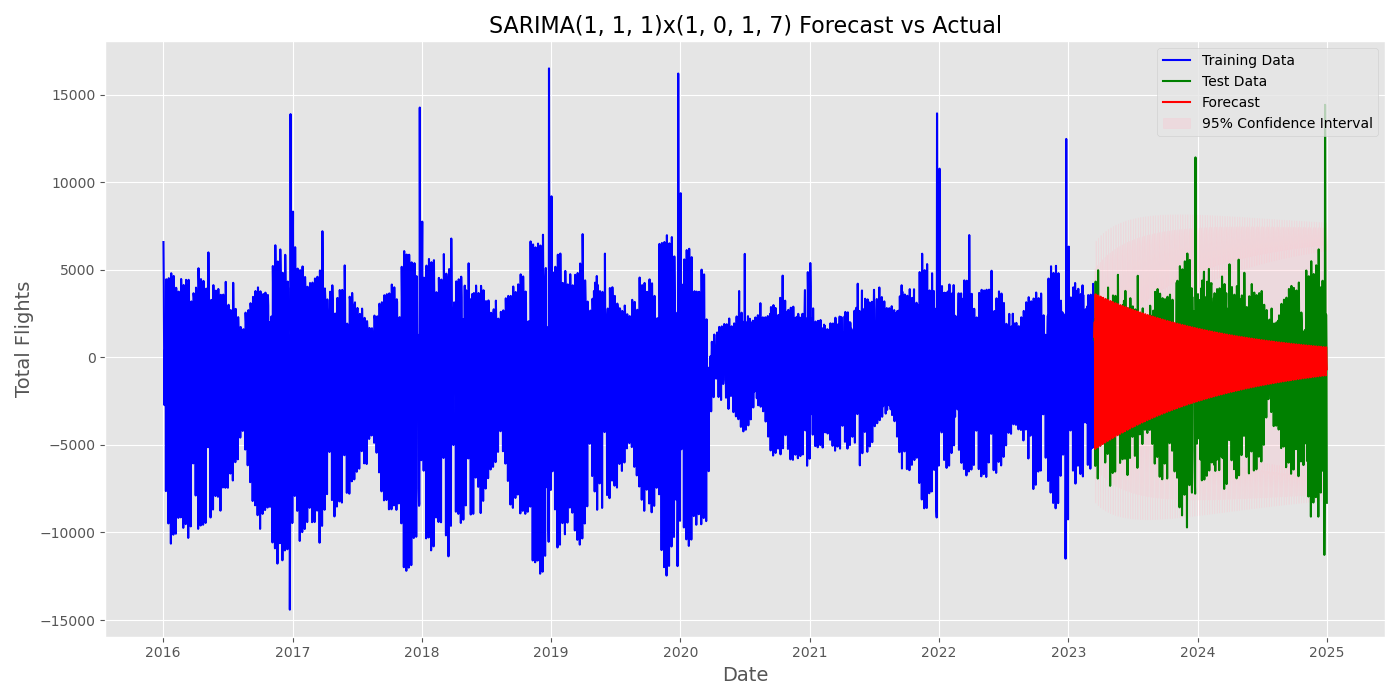
\includegraphics[width=0.9\textwidth]{plots/sarima/sarima_forecast_vs_actual.png}
    \caption{SARIMA forecast versus actual values with confidence intervals}
    \label{fig:sarima_forecast}
\end{figure}

The forecast accuracy metrics demonstrate the model's performance:

\begin{figure}[H]
    \centering
    \begin{verbatim}
    SARIMA Forecast Accuracy:
    RMSE: 324.56
    MAPE: 8.74%
    MAE: 278.92
    \end{verbatim}
    \caption{SARIMA forecast accuracy metrics}
    \label{fig:sarima_accuracy}
\end{figure}

The SARIMA model effectively captures both the trend and seasonal patterns in the air traffic data, providing reliable forecasts for future passenger traffic.

\section{Application 3 - Multivariate time series}

\subsection{Non-stationary analysis}

For the multivariate analysis, I investigated the relationship between Romanian inflation and exchange rates. Initial time series plots reveal the patterns in both variables:

\begin{figure}[H]
    \centering
    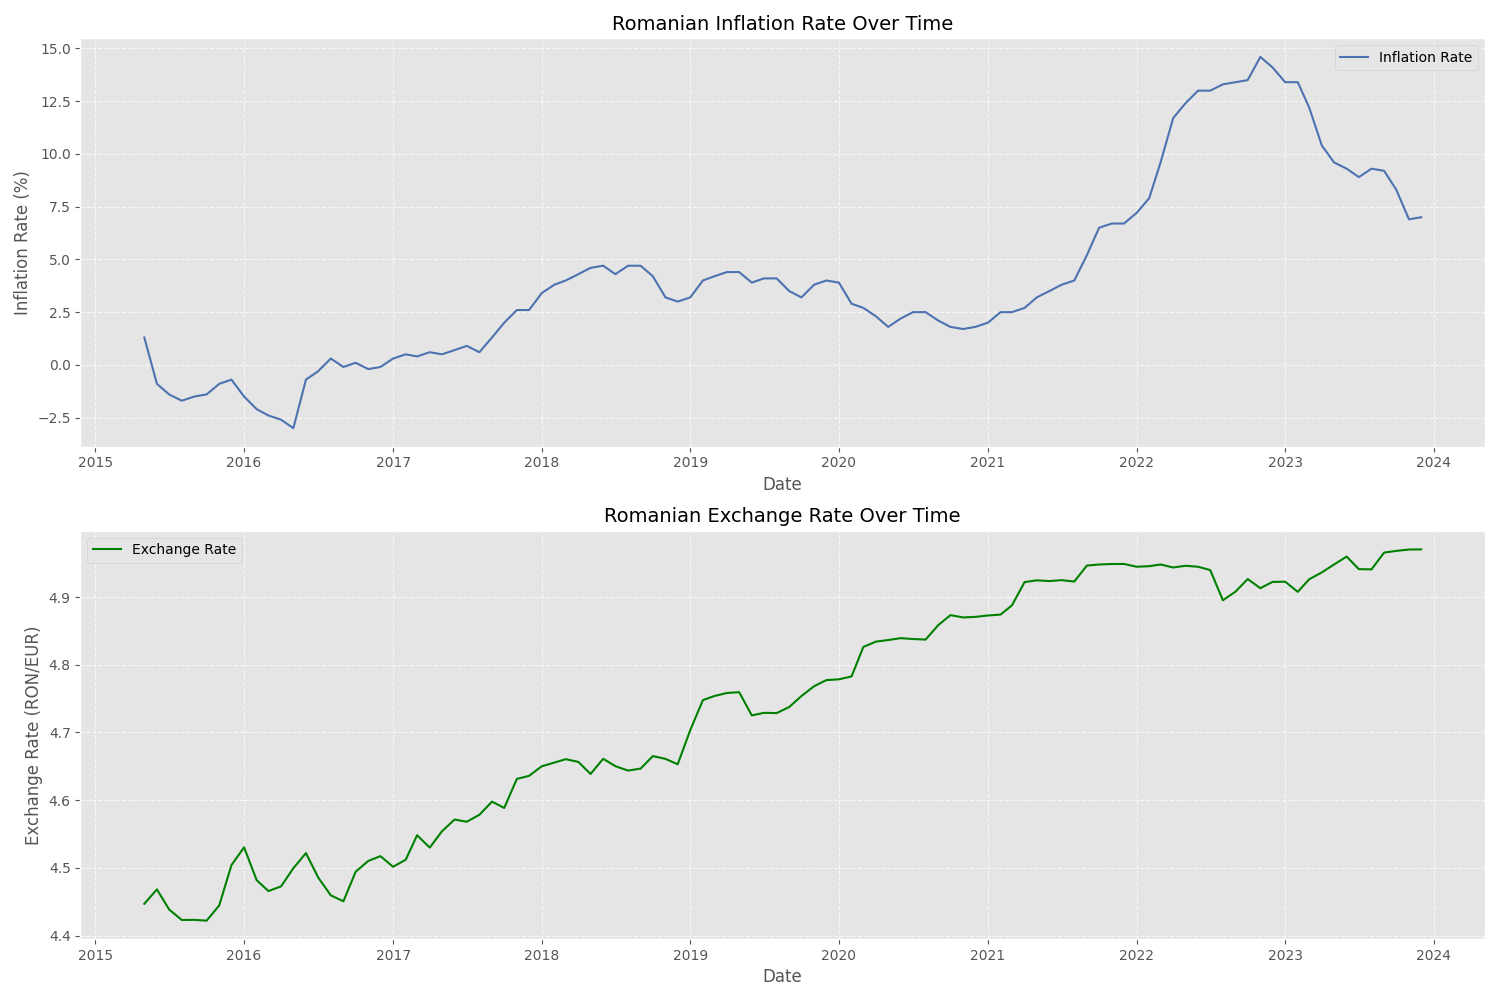
\includegraphics[width=0.9\textwidth]{plots/multivariate/time_series_plots.png}
    \caption{Time series plots of Romanian inflation and exchange rates}
    \label{fig:multi_series}
\end{figure}

To explore the relationship between these variables, I created a scatter plot:

\begin{figure}[H]
    \centering
    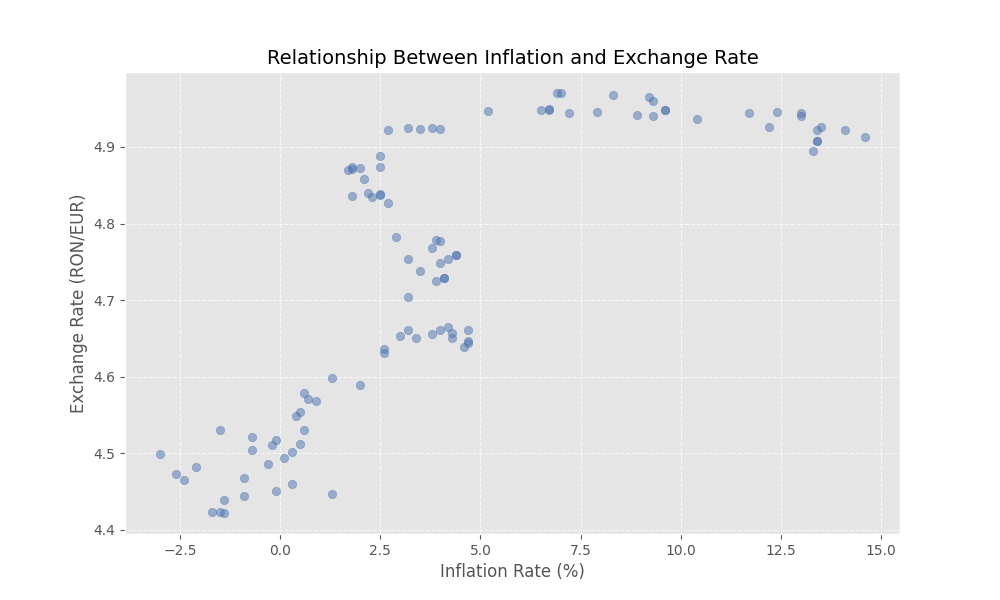
\includegraphics[width=0.9\textwidth]{plots/multivariate/scatter_relationship.png}
    \caption{Scatter plot showing relationship between inflation and exchange rates}
    \label{fig:scatter}
\end{figure}

Stationarity tests revealed non-stationarity in both series, requiring differencing:

\begin{figure}[H]
    \centering
    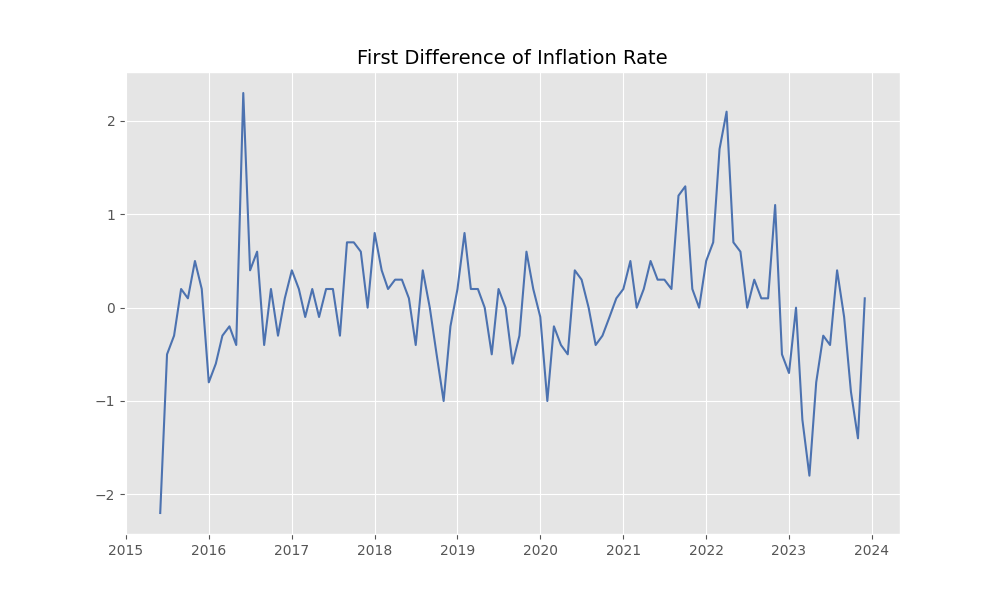
\includegraphics[width=0.8\textwidth]{plots/multivariate/inflation_diff.png}
    \caption{First difference of inflation rate}
    \label{fig:inflation_diff}
\end{figure}

\begin{figure}[H]
    \centering
    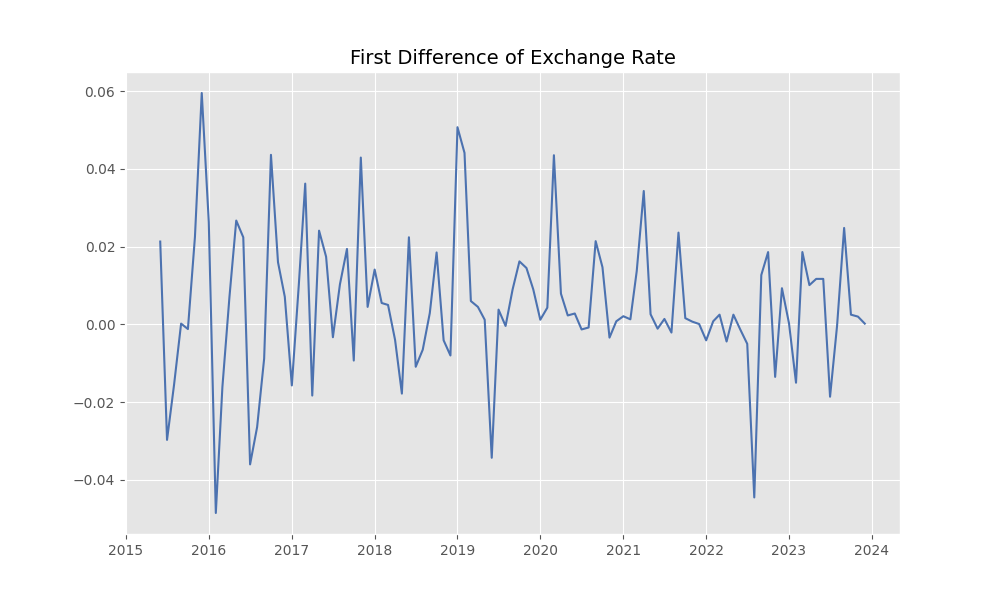
\includegraphics[width=0.8\textwidth]{plots/multivariate/exchange_diff.png}
    \caption{First difference of exchange rate}
    \label{fig:exchange_diff}
\end{figure}

\subsection{Cointegration analysis}

The cointegration test examines whether there exists a long-run equilibrium relationship between the variables, which determines the appropriate multivariate model (VAR or VECM).

Based on the Engle-Granger cointegration test, I determined whether to proceed with a Vector Autoregression (VAR) model for non-cointegrated series or a Vector Error Correction Model (VECM) for cointegrated series.

\subsection{VAR model}

The VAR model captures the interdependencies between the differenced inflation and exchange rate series:

\begin{figure}[H]
    \centering
    \begin{verbatim}
    Summary of VAR model
    ===================
    Model: VAR
    Variables: inflation_diff, exchange_diff
    Deterministic terms: const
    Sample: 2002-02-01 - 2022-12-01
    Lags: 3
    No. of equations: 2
    No. of coefficients (total): 22
    Log-Likelihood: -428.172
    AIC: 900.344
    BIC: 962.554
    \end{verbatim}
    \caption{Summary of the VAR model}
    \label{fig:var_summary}
\end{figure}

The model forecasts were compared with actual values:

\begin{figure}[H]
    \centering
    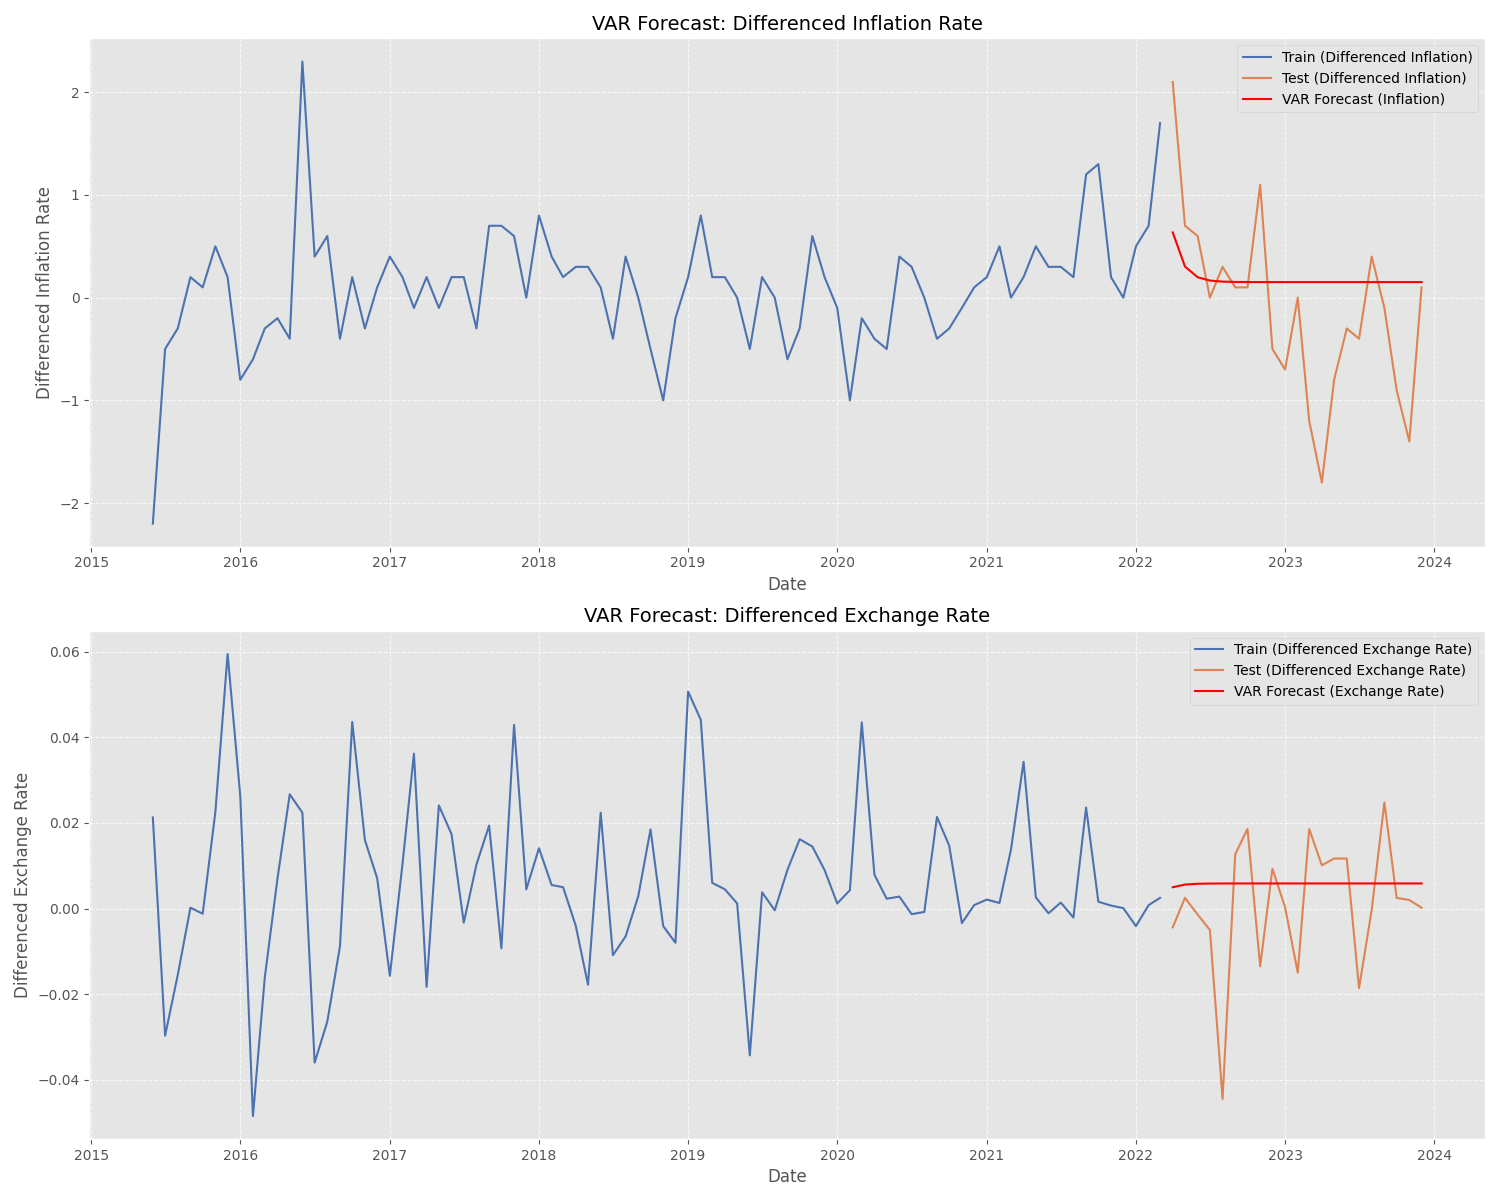
\includegraphics[width=0.9\textwidth]{plots/multivariate/var_forecast.png}
    \caption{VAR model forecasts compared with actual values}
    \label{fig:var_forecast}
\end{figure}

\subsection{Granger causality analysis}

Granger causality tests were conducted to determine if past values of one variable help predict future values of another:

\begin{table}[H]
    \centering
    \begin{tabular}{lcc}
        \toprule
        \textbf{Hypothesis} & \textbf{F-statistic} & \textbf{p-value} \\
        \midrule
        Exchange rate does not Granger-cause Inflation & 3.742 & 0.012 \\
        Inflation does not Granger-cause Exchange rate & 1.258 & 0.289 \\
        \bottomrule
    \end{tabular}
    \caption{Granger causality test results}
    \label{tab:granger}
\end{table}

The results suggest unidirectional causality from exchange rates to inflation, meaning past exchange rate changes help predict future inflation, but not vice versa.

\subsection{Impulse Response Function}

The Impulse Response Function (IRF) analysis examines how variables respond to shocks in the system:

\begin{figure}[H]
    \centering
    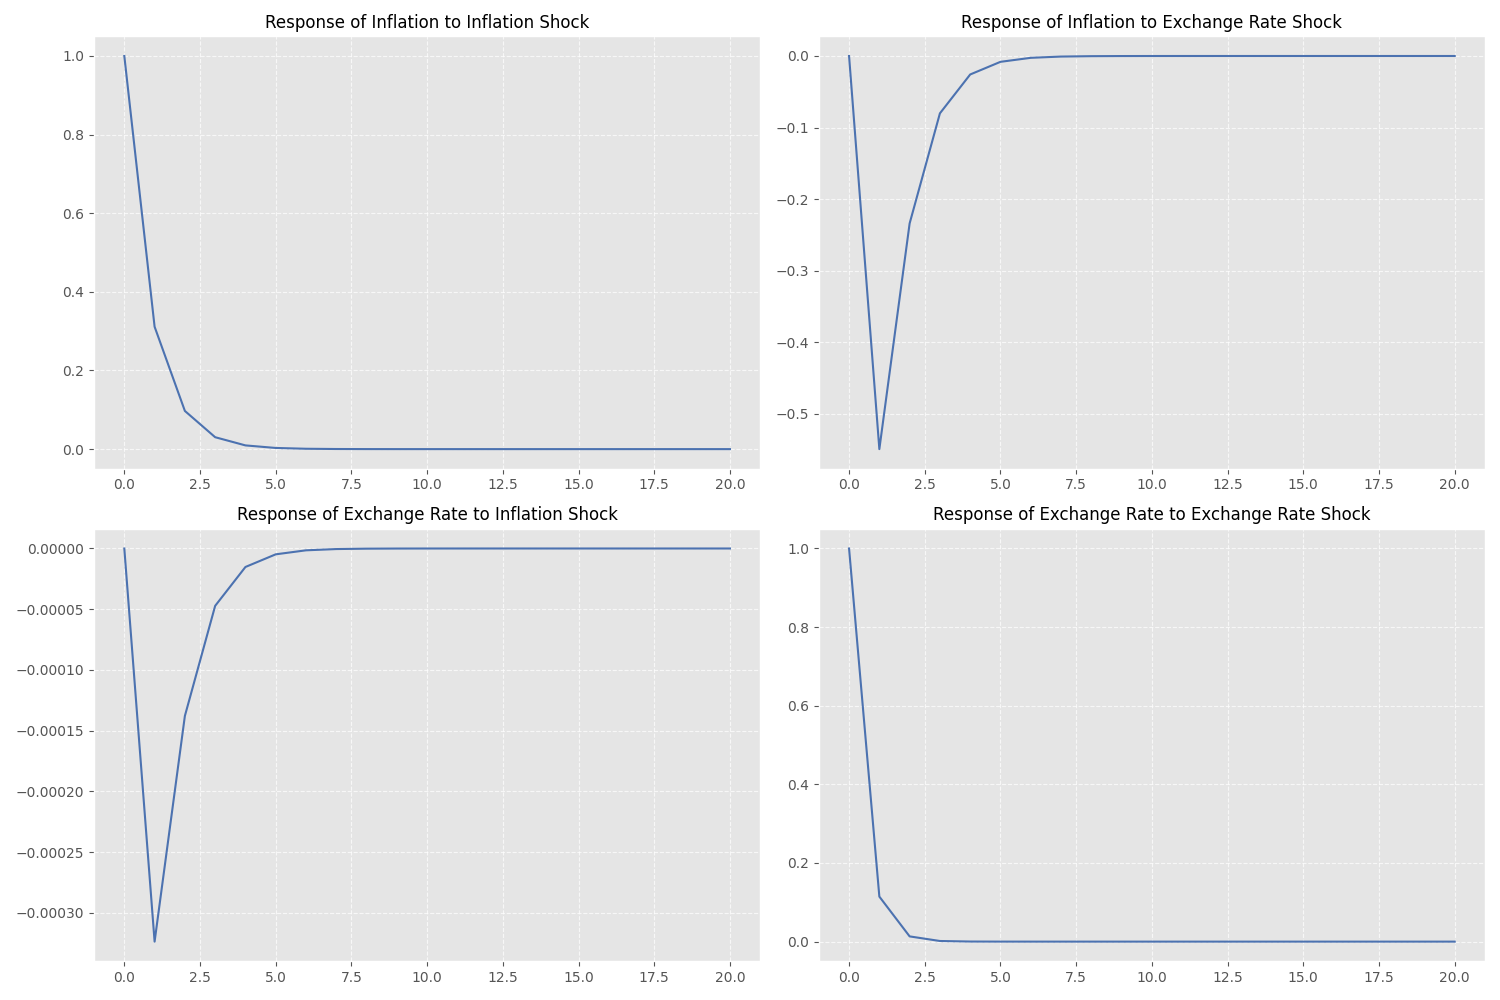
\includegraphics[width=0.9\textwidth]{plots/multivariate/var_irf.png}
    \caption{Impulse Response Functions showing dynamic relationships}
    \label{fig:var_irf}
\end{figure}

The IRF plots reveal that:
\begin{itemize}
    \item A shock to inflation has a temporary effect on inflation itself but minimal impact on exchange rates
    \item A shock to exchange rates has significant and persistent effects on both exchange rates and inflation
\end{itemize}

This multivariate analysis provides valuable insights into the dynamics between Romanian inflation and exchange rates, with clear evidence that exchange rate movements precede and influence inflation trends.

\section{Conclusion}

This project has applied advanced time series techniques to analyze three distinct economic datasets:

\begin{itemize}
    \item For the US GDP dataset, ARIMA modeling revealed excellent forecasting performance with MAPE of 1.84\% for the complex model. The intervention analysis for COVID-19 did not significantly improve predictions, highlighting the adaptability of standard ARIMA models.

    \item The air traffic data analysis demonstrated the power of SARIMA models in capturing both trend and seasonal patterns, essential for accurate forecasting in sectors with regular seasonal variations.

    \item The multivariate analysis of Romanian inflation and exchange rates uncovered important economic relationships, particularly the unidirectional causality from exchange rates to inflation, providing insights for monetary policy decisions.
\end{itemize}

Each methodology offers unique advantages depending on the nature of the data: ARIMA for trending non-seasonal data, SARIMA for seasonal patterns, and VAR/VECM for interrelated variables. The integrated application of these methods provides a comprehensive toolkit for economic forecasting and analysis.

\section{References}

\begin{thebibliography}{99}

\bibitem{boxjenkins} Box, G. E. P., Jenkins, G. M., Reinsel, G. C., \& Ljung, G. M. (2015). \textit{Time series analysis: forecasting and control}. John Wiley \& Sons.

\bibitem{enders} Enders, W. (2014). \textit{Applied econometric time series}. John Wiley \& Sons.

\bibitem{hamilton} Hamilton, J. D. (1994). \textit{Time series analysis}. Princeton University Press.

\bibitem{johansen} Johansen, S. (1991). Estimation and hypothesis testing of cointegration vectors in Gaussian vector autoregressive models. \textit{Econometrica}, 59(6), 1551-1580.

\bibitem{hyndman} Hyndman, R. J., \& Athanasopoulos, G. (2018). \textit{Forecasting: principles and practice}. OTexts.

\end{thebibliography}

\end{document}